\documentclass[9pt]{beamer}
\usepackage{tikz}
\usepackage{subfiles}
\usepackage{graphicx} 
\usepackage{hyperref}
\usepackage{multimedia}
\usepackage{subcaption}
%\usepackage[table,xcdraw]{xcolor}  %to include tables with colors
\usepackage{comment}

\setbeamertemplate{footline}[page number]
\mode<presentation>{
%\usetheme{Malmoe}
%\usetheme{Antibes}
%\usetheme{warsaw}
\usetheme{Frankfurt}  %%
%\usetheme{Dresden}
%\usetheme{Madrid}
%\usetheme{Malmoe} %
%\usetheme{Ilmenau}
}
%\setbeamertemplate{footline}[\insertframenumber]

%\newcommand*\oldmacro{}%
%\let\oldmacro\insertshorttitle%
%\renewcommand*\insertshorttitle{%
% \oldmacro\hfill%
% \insertframenumber\,/\,\inserttotlaframenumber}

\AtBeginSection[]
{
\begin{frame}<beamer>
\frametitle{Plan}
\tableofcontents[currentsection]
\end{frame}
}




\makeatletter
\let\insertsupervisor\relax
\newcommand\supervisortitle{Supervisor }
\makeatletter
\let\insertsupervisorinst\relax
\newcommand\supervisorinsttitle{Supervisorinst}
\mode<all>
{
  \newcommand\supervisor[1]{\def\insertsupervisor{#1}}
  \titlegraphic{}
}
\mode<all>
{
  \newcommand\supervisorinst[1]{\def\insertsupervisorinst{#1}}
  \titlegraphic{}
}
\defbeamertemplate*{title page}{supdefault}[1][]
{
  \vbox{}
  \vfill
  \begingroup
    \centering
    \begin{beamercolorbox}[sep=8pt,center,#1]{title}
%      \usebeamerfont{title}
      \inserttitle\par%
      \ifx\insertsubtitle\@empty\relax%
      \else%
        \vskip0.25em%
        {%\usebeamerfont{subtitle}
        \usebeamercolor[fg]{subtitle}\insertsubtitle\par}%
      \fi%     
    \end{beamercolorbox}%
    \vskip1em\par
    \begin{beamercolorbox}[sep=8pt,center,#1]{author}
    Presented By:\\
%      \usebeamerfont{author}
      \textbf{\insertauthor} \\
%      \usebeamerfont{institute}
      \insertinstitute
    \end{beamercolorbox}
   %     \begin{beamercolorbox}{institute}
   %   \usebeamerfont{institute}\insertinstitute
   % \end{beamercolorbox}
    \ifx\insertsupervisor\relax\relax\else
    \begin{beamercolorbox}[sep=8pt,center,#1]{author}
%      \usebeamerfont{author}
      \supervisortitle: \\ \textbf{~\insertsupervisor} \\
%      \usebeamerfont{institute}
      \insertsupervisorinst
    \end{beamercolorbox}\fi
    %\begin{beamercolorbox}[sep=8pt,center,#1]{institute}
    %  \usebeamerfont{institute}\insertinstitute
    %\end{beamercolorbox}
    \begin{beamercolorbox}[sep=8pt,center,#1]{date}
%      \usebeamerfont{date}
      \insertdate
    \end{beamercolorbox}\vskip0.5em
    {\usebeamercolor[fg]{titlegraphic}\inserttitlegraphic\par}
  \endgroup
  \vfill
}
\setbeamertemplate{title page}[supdefault][colsep=-4bp,rounded=true,shadow=\beamer@themerounded@shadow]\makeatother

\title{Finite Element simulation of 2D metal strip in Hot-Dip galvanization Process}
%\subtitle{Reissner Mindlin Plate}
\author{Emayavaramban ELANGO}
\supervisor{PHAM Van Thang}
\supervisorinst{PHAM Van Thang }
\institute{\'Ecole centrale De Nantes}
\supervisorinst{ArcelorMittal Maizi\`eres Research SA }
\date{\today}


\begin{document}
%\title[Finite Element simulation of 2D metal strip in Hot-Dip galvanization Process]{FEM in plates}
%\author{Emayavaramban Elango}
%\institute[ECN]


\begin{frame}
\maketitle
\end{frame}


\begin{frame}
\frametitle{Table of Content}
\tableofcontents
\end{frame}
\section{Introduction}

\begin{frame}
%\frametitle{Plan}
\begin{figure}[h!]
%\centering
%\minipage{1\textwidth}%
  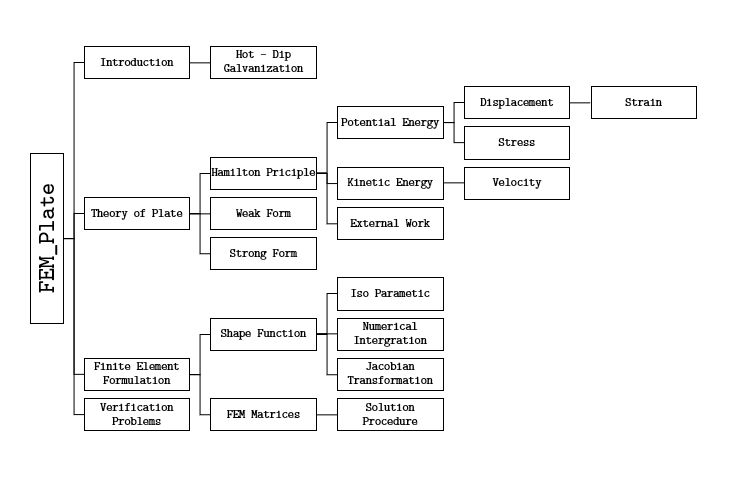
\includegraphics[width=1\linewidth,trim={0 0 0 1cm},clip]{tree.png}
 % \caption{FEM solution plot}\label{fig:awesome_image3}
%\endminipage
\end{figure}
\end{frame}


\subsection{Hot-Dip Galvanization Process}
\begin{frame}
\frametitle{Hot-Dip Galvanization Process}
\begin{columns}
\column{0.5\textwidth}

\begin{figure}[h!]
%\centering
%\minipage{1\textwidth}%
  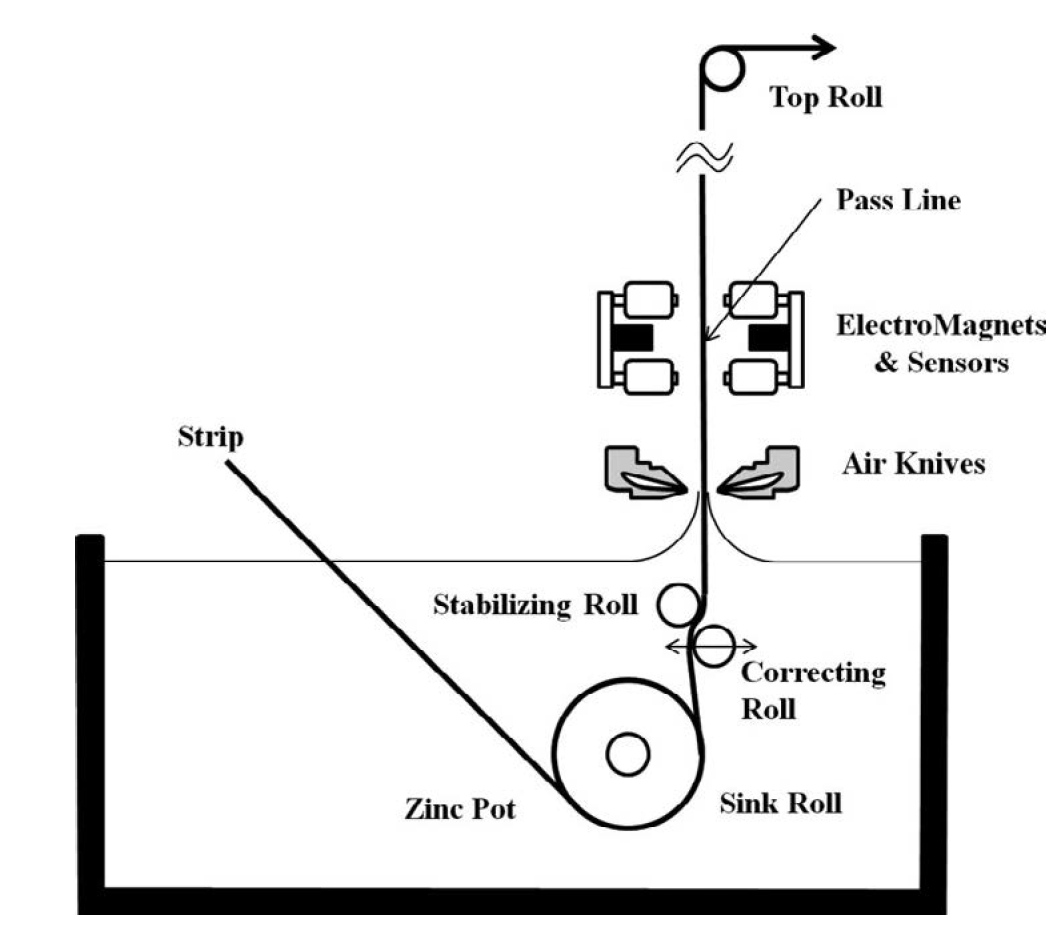
\includegraphics[width=1\linewidth,trim={0 0 0 1cm},clip]{hotdip.png}
 % \caption{FEM solution plot}\label{fig:awesome_image3}
%\endminipage
\end{figure}
\column{0.5\textwidth}
\begin{itemize}
\item A thin Layer of Zinc is coated to Increase the corrosion resistance of steel
\item Air knives control the thickness of the Zinc layer
\item Excessive Vibration results in uneven coating.
\item Electromagnets are used to control the  vibration of the strip. 
\end{itemize}
\end{columns}
\end{frame}




\begin{frame}
\frametitle{Need For Finite Element Modeling}

\begin{itemize}
\item Complex behavior of the metal strip.
\item Two dimensional domain and Three Dimensional Displacement field.
\item Complex and multiple boundary condition.
\item Free Control over discretization of the domain.
\item Intuitive Solution Procedure.
\end{itemize}

\end{frame}

\section{Theory of Plates}
\begin{frame}
\frametitle{Theory of Plates (Reissner-Mindlin Plate Theory)}
A plate is a flat solid with uniform and smaller thickness than its other dimensions.A middle plane (Z=0) is equidistant from upper and lower faces.
\begin{block}{Assumptions (Thin and Thick Plate)}
\begin{itemize}
\item A point in the middle plane only moves vertically $u = 0$ and $v = 0 $
\item Thickness does not change during deformation.
\item only $\sigma_{33}$ is neglected (plane stress is assumed)
\item A line normal to the undeformed middle plane remains straight and not necessarily normal after deformation.
\end{itemize}
\end{block}


\begin{columns}
\column{0.5\textwidth}
\begin{figure}[h!]
%\centering
%\minipage{1\textwidth}%
  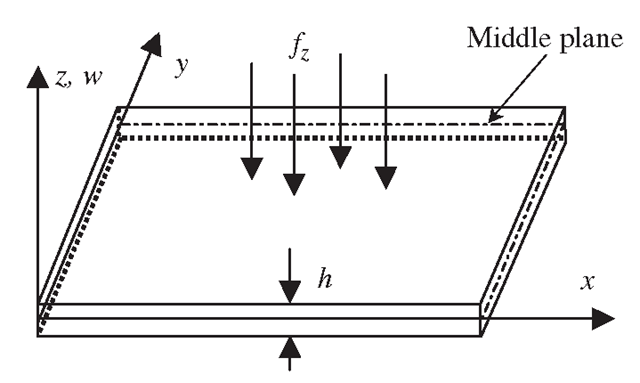
\includegraphics[width=1\linewidth,trim={0 0 0 1cm},clip]{plate.png}
 % \caption{FEM solution plot}\label{fig:awesome_image3}
%\endminipage
\end{figure}

\column{0.5\textwidth}


\begin{figure}[h!]
%\centering
%\minipage{1\textwidth}%
  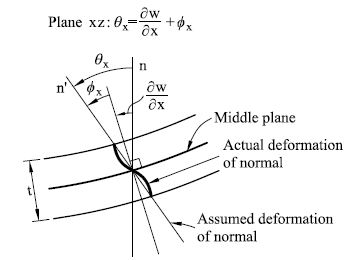
\includegraphics[width=1\linewidth,trim={0 0 0 0},clip]{RMplate.png}
 % \caption{FEM solution plot}\label{fig:awesome_image3}
%\endminipage
\end{figure}


\end{columns}

\end{frame}


\begin{comment}

\begin{frame}
\frametitle{Theory of Plates}
\begin{block}{Kirchhoff Plate Theory}
\begin{itemize}
\item A line normal to the undeformed middle plane remains straight and normal after deformation.
\item Only for \textbf{Thin Plates} where $t/a \leq 0.1 $.
\item $\sigma_{23}$ and $\sigma_{13}$ are neglected.
\end{itemize}
\end{block}


\begin{figure}[h!]
%\centering
%\minipage{1\textwidth}%
  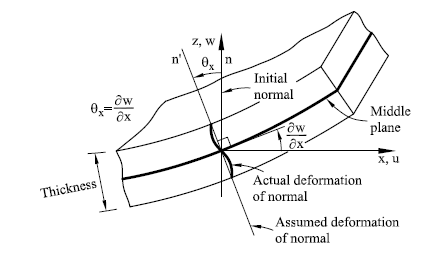
\includegraphics[width=0.6\linewidth,trim={0 0 0 0},clip]{Kplate.png}
 % \caption{FEM solution plot}\label{fig:awesome_image3}
%\endminipage
\end{figure}

\end{frame}


\begin{frame}
\frametitle{Theory of Plates (Reissner-Mindlin Plate Theory)}

\begin{block}{Reissner-Mindlin Plate Theory ( \textbf{Thin and Thin Plates} ) }
\begin{itemize}
\item A line normal to the undeformed middle plane remains straight and not necessarily normal after deformation.
\item For both \textbf{Thin and Thin Plates}.
%\item $\sigma_{23}$ and $\sigma_{13}$ are not neglected.
\end{itemize}
\end{block}


\begin{figure}[h!]
%\centering
%\minipage{1\textwidth}%
  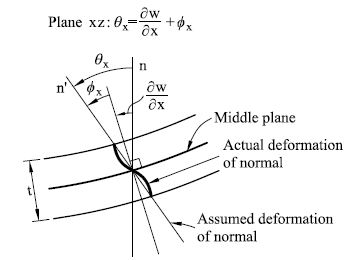
\includegraphics[width=0.6\linewidth,trim={0 0 0 0},clip]{RMplate.png}
 % \caption{FEM solution plot}\label{fig:awesome_image3}
%\endminipage
\end{figure}

\end{frame}

\end{comment}


\begin{frame}
\frametitle{Description of Domain}

\begin{figure}[h!]
\centering
\subfile{domain.tex}
%\caption{NAS277} \label{NAS277sch}
\end{figure}
\begin{itemize}

\item $\Omega$ is the two dimensional domain strictly in xy plane 
\item $h$ is the thickness of the plate 
\item $\Omega_1$...$\Omega_i$ are the sub-domains where pressure forces $q_1$..$q_i$ are applied
\item $V$ is the Line speed and  $Nx$ is the tension on the line
\item $L$ is the length and  $W$ is the width 

\end{itemize}

\end{frame}

\subsection{Hamilton Principle}
\begin{frame}
\frametitle{Hamilton principle}
Hamilton principle is used to derive the equation of motion. 
and the Hamilton is given as 
 \begin{align*}
H  = \int_{t_0}^{t_1} \left( T - V + W \right) dt  
 \end{align*}
 The Hamilton Principle states that variation of Hamilton is zero
 \begin{align*}
 \delta H  =  \int_{t_0}^{t_1} \left( \delta T - \delta V + \delta W \right) dt     =  0 
 \end{align*}
 The variation of displacement $\delta u$ is zero at the beginning and end time.
 \begin{align*}
 \delta u \Big|_{t_0}^{t_1} = 0
 \end{align*}
 $T$ is the kinetic energy, $V$ in the potential energy and $W$ is the work done to the system.
 
\end{frame}
\subsection{Potential Energy}
\begin{frame}
\frametitle {Potential Energy}
The Total Potential energy of the domain is given as 
\begin{equation*}
V=\frac{1}{2}\int\int\int_\Gamma \epsilon^T \sigma  d \Gamma
\end{equation*}
$\epsilon$ and $\sigma$ are strain and stress respectively. The Potential Energy is separated into Bending ($B$) , Shear ($S$) and Axial ($A$) component.
\begin{equation*}
V=\frac{1}{2}\int\int\int_\Gamma \left(\epsilon^B\right)^T \sigma^B + \left(\epsilon^S\right)^T \sigma^S + \left(\epsilon^A\right)^T \sigma^A d \Gamma
\end{equation*}
Since Thickness is constant and continuous it is integrated now.
\begin{equation*}
V=\frac{1}{2}\int\int_\Omega \int_{-h/2}^{+h/2} \left(\epsilon^B\right)^T \sigma^B + \left(\epsilon^S\right)^T \sigma^S + \left(\epsilon^A\right)^T \sigma^A dz d \Omega
\end{equation*}

%$\epsilon^B$ is the stress due to bending, $\epsilon^S$ is the stress due to shear deformation and  $\epsilon^A$ is the axial stress.
Which gives us
\begin{equation*}
\begin{split}
V=\frac{1}{2} \int\int_\Omega \kappa^T \tilde{\sigma}^B 
+ \left({\epsilon}^S\right)^T \tilde{\sigma}^S 
+ \left({\epsilon}^A\right)^T \tilde{\sigma}^A  d \Omega
\end{split}
\end{equation*}


\end{frame}

\begin{frame}

\frametitle{Strain}
Using the plate theory, each strain components is given as 
\begin{align*}
\epsilon^B & = -z
\begin{bmatrix}
\dfrac{\partial w^2 }{\partial x^2}
\\
\dfrac{\partial w^2 }{\partial y^2}
\\
\dfrac{\partial w^2 }{\partial x \partial y}
\end{bmatrix}
=-z \kappa = -z \mathbf{\triangle} w 
\\
\epsilon^A &
=
\frac{1}{2}
\begin{bmatrix}
\dfrac{\partial w}{\partial x} \\
\dfrac{\partial w}{\partial y}
\end{bmatrix}
\begin{bmatrix}
\dfrac{\partial w}{\partial x} &
\dfrac{\partial w}{\partial y}
\end{bmatrix}
=
\frac{1}{2}
w_{, \alpha}w_{, \beta}  \qquad  \alpha,\beta \in x,y
\\
\epsilon^S & = \dfrac{1}{2}
\begin{bmatrix}
\dfrac{\partial w}{\partial x}-\theta_x 
\\
\dfrac{\partial w}{\partial y}-\theta_y 
\end{bmatrix} 
=
\frac{1}{2} \left( w_{,\alpha}-\theta_{\alpha}  \right)
\end{align*}




\end{frame}


\begin{frame}
\frametitle{Stress}
For \textbf{Linear Isotropic} material the corresponding stress strain relation is given as
\begin{equation*}
\tilde{\sigma}^B = \begin{bmatrix}
\sigma_{11}
\\
\sigma_{22}
\\
2 \sigma_{12}
\end{bmatrix}
=\dfrac{Eh^3}{1-\nu^2}
\begin{bmatrix}
1 & \nu  & 0
\\
\nu  & 1 & 0
\\
0 & 0 & (1-\nu)
\end{bmatrix}
\begin{bmatrix}
\epsilon_{11}
\\
\epsilon_{22}
\\
2 \epsilon_{12}
\end{bmatrix}
=
\tilde{\mathbf{D}} \kappa
\end{equation*}


The shear stress and strain relation from the 3D constitutive law is given as
\begin{equation*}
\tilde{\sigma}^S = \begin{bmatrix}
2 \sigma_{31}
\\
2 \sigma_{32}
\end{bmatrix}
=Gh
\begin{bmatrix}
1 & 0 
\\
0 & 1 
\end{bmatrix}
\begin{bmatrix}
2\epsilon_{31}
\\
2\epsilon_{32}
\end{bmatrix}
=
\tilde{\mathbf{D}}_c
\sigma^S
\end{equation*}

Axial is stress is provided and it is considered as constant and uniform over the domain.

\begin{equation*}
\tilde{\sigma}^A = \begin{bmatrix}
\tilde{\sigma}_{11} & \tilde{\sigma}_{12}
\\
\tilde{\sigma}_{12} & \tilde{\sigma}_{22}
\end{bmatrix}
=h
\begin{bmatrix}
N_x & N_{xy}
\\
N_{xy} & N_y
\end{bmatrix}
\end{equation*}


$E$ is the Young's modulus, $\nu$ is the Poisson's ratio and $G$ is the shear modulus which is given by $G=E / 1+\nu $. 
\end{frame}


\begin{comment}





\begin{frame}
\frametitle{Kinematics}
\begin{align*}
u_1 \left( x, y ,z,t\right) & =  u \left( x ,y,t\right) - z \theta_x \left(x,y,t\right) & \theta_x  = \frac{\partial w }{\partial x} + \phi_x \\
u_2 \left( x, y ,z,t\right) & =  v \left( x, y ,t\right) - z \theta_y \left(x,y,t\right)& \theta_y  = \frac{\partial w }{\partial y} + \phi_y\\
u_3 \left( x, y ,z,t\right) & =  w \left(x, y ,t\right) 
\end{align*}
\begin{columns}
\column{0.65\textwidth}
\begin{equation*}
\left\{
\begin{array}{r}
 u_1 \\ u_2 \\ u_3  
\end{array}
\right\}
=
\begin{bmatrix}
z & 0 & 0 \\
0 & z & 0 \\
0 & 0 & 1 \\
\end{bmatrix}
\left\{
\begin{array}{r}
 \theta_x \\ \theta_y \\ w 
\end{array}
\right\}
=
\left[Z \right] \tilde{u}
\end{equation*}
\column{0.35\textwidth}
\begin{figure}[h!]
%\centering
%\minipage{1\textwidth}%
  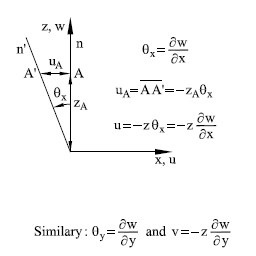
\includegraphics[width=1\linewidth,trim={0 2cm 0 0},clip]{displacement.png}
 % \caption{FEM solution plot}\label{fig:awesome_image3}
%\endminipage
\end{figure}
\end{columns}

\end{frame}


\begin{frame}
\frametitle{Strain Definition}
The Green - Lagrange strain tensor is given as
\begin{equation*}
\epsilon_{ij} = \frac{1}{2} \left(  u_{i,j} +  u_{j,i} + u_{k,i}u_{k,j} \right) \qquad i,j \in 1,2,3
\end{equation*}


The $E_{11}$ component of the strain tensor is found as
\begin{align*}
E_{11} = -z \dfrac{\partial w^2 }{\partial x^2} + \dfrac{1}{2}\left(\left[z\dfrac{\partial \theta_x}{\partial x}\right] ^2 +z^2 \dfrac{\partial \theta_y}{\partial x}\dfrac{\partial \theta_y}{\partial y} + \dfrac{\partial w}{\partial x} \dfrac{\partial w}{\partial x}\right)
\end{align*}

\begin{align*}
E_{11} = -z \dfrac{\partial w^2 }{\partial x^2} + \dfrac{1}{2} \left( \dfrac{\partial w}{\partial x} \right)^2
\end{align*}
\end{frame}

\begin{frame}
\begin{align*}
E_{i,j} =  
\begin{bmatrix}
 -z \dfrac{\partial w^2 }{\partial x^2} + \dfrac{1}{2} \left( \dfrac{\partial w}{\partial x} \right)^2
 & 
 -z \dfrac{\partial w^2 }{\partial x \partial y} + \dfrac{1}{2}  \dfrac{\partial w}{\partial x} \dfrac{\partial w}{\partial y} 
 & 
 \dfrac{1}{2} \left( \dfrac{\partial w}{\partial x}-\theta_x \right)
 \\
 &
 -z \dfrac{\partial w^2 }{\partial y^2} + \dfrac{1}{2} \left( \dfrac{\partial w}{\partial y} \right)^2
 &
  \dfrac{1}{2} \left( \dfrac{\partial w}{\partial y}-\theta_y \right)
  \\
  symm.
  &
  &
  0
\end{bmatrix}
\end{align*}



\begin{align*}
\epsilon_{\alpha \beta}^B = -z
\begin{bmatrix}
\dfrac{\partial w^2 }{\partial x^2}
\\
\dfrac{\partial w^2 }{\partial y^2}
\\
\dfrac{\partial w^2 }{\partial x \partial y}
\end{bmatrix}
=-z \kappa
  \quad  \alpha,\beta\in 1,2
\end{align*}
$\kappa= \mathbf{\triangledown} w$ is the curvature of of a plane.
\end{frame}
\begin{frame}
\begin{columns}
\column{0.5\textwidth}
For Kirchhoff plate
\begin{align*}
\epsilon_{3\alpha}^S =
\begin{bmatrix}
0
\\
0 
\end{bmatrix} 
\end{align*}
\column{0.5\textwidth}
For Reissner - Mindlin Plate
\begin{align*}
\epsilon_{3\alpha}^S = \dfrac{1}{2}
\begin{bmatrix}
-\phi_x 
\\
-\phi_y 
\end{bmatrix} 
\end{align*}
\end{columns}
\end{frame}

\begin{frame}
\frametitle{Constitute law}
For the \textbf{linear isotropic} material is considered. Since $\sigma_{33}$ is not considered the \textbf{plane stress} case is considered and the stress - strain relation is given as
\begin{equation*}
\sigma_{\alpha\beta}^B = \begin{bmatrix}
\sigma_{11}
\\
\sigma_{22}
\\
2 \sigma_{12}
\end{bmatrix}
=\dfrac{1}{1-\nu^2}
\begin{bmatrix}
E & \nu E & 0
\\
\nu E & E & 0
\\
0 & 0 & (1-\nu^2)G
\end{bmatrix}
\begin{bmatrix}
\epsilon_{11}
\\
\epsilon_{22}
\\
2 \epsilon_{12}
\end{bmatrix}
\end{equation*}



$E$ is the Young's modulus, $\nu$ is the Poisson's ratio and $G$ is the shear modulus which is given by $G=E / 1+\nu $. 
\begin{equation*}
\sigma_{\alpha\beta}^B = \mathbf{D} \epsilon_{\alpha\beta}^B
\end{equation*}
\end{frame}


\begin{frame}

The shear stress and strain relation from the 3D constitutive law is given as
\begin{equation*}
\sigma_{3\alpha}^S = \begin{bmatrix}
2 \sigma_{31}
\\
2 \sigma_{32}
\end{bmatrix}
=G
\begin{bmatrix}
1 & 0 
\\
0 & 1 
\end{bmatrix}
\begin{bmatrix}
2\epsilon_{31}
\\
2\epsilon_{32}
\end{bmatrix}
=
\mathbf{D_c}
\sigma_{3\alpha}^S
\end{equation*}

Axial is stress is provided and it is considered as constant and uniform over the domain.

\begin{equation*}
\sigma_{\alpha\beta}^A = \begin{bmatrix}
\sigma_{11} & \sigma_{12}
\\
\sigma_{12} & \sigma_{22}
\end{bmatrix}
=
\begin{bmatrix}
N_x & N_{xy}
\\
N_{xy} & N_y
\end{bmatrix}
=
N
\end{equation*}

\end{frame}
\end{comment}
\begin{frame}
\frametitle{variation of Potential Energy}

Potential Energy equation is written again

\begin{equation*}
\begin{split}
V=\frac{1}{2} \int\int_\Omega \kappa^T \tilde{\sigma}^B 
+ \left({\epsilon}^S\right)^T \tilde{\sigma}^S 
+ \left({\epsilon}^A\right)^T \tilde{\sigma}^A  d \Omega
\end{split}
\end{equation*}

Now the strain and stress are substituted in the Potential equation


\begin{equation*}
\begin{split}
V=\frac{1}{2} \int\int_\Omega  \kappa^T \tilde{D}  \kappa 
+ \left({\epsilon}^S\right)^T {\tilde{D}_c}{\epsilon}^S 
+ w_{, \alpha} \tilde{\sigma}^A w_{, \beta}  d \Omega
\end{split}
\end{equation*}

finally taking the variation gives us
\begin{block}{Variation of Total Potential Energy}
\begin{equation*}
\begin{split}
\delta V=\int\int_\Omega  \kappa^T \tilde{D}  \delta \kappa 
+ \left({\epsilon}^S\right)^T {\tilde{D}_c}  \delta {\epsilon}^S 
+ w_{, \alpha} \tilde{\sigma}^A  \delta w_{, \alpha}  d \Omega
\end{split}
\end{equation*}

\end{block}

\end{frame}
\begin{comment}


\begin{frame}

\begin{equation*}
\begin{split}
\delta V=\int\int_\Omega  \kappa^T \tilde{D}  \delta \kappa 
+ \left(\tilde{\epsilon}^S\right)^T {\tilde{D}_c}  \delta \tilde{\epsilon}^S 
+ \frac{1}{2} \left( \delta  \tilde{\epsilon}^A\right)^T \tilde{\sigma}^A  d \Omega
\end{split}
\end{equation*}


\begin{equation*}
\frac{1}{2} \left( \delta  \tilde{\epsilon}^A\right)^T \tilde{\sigma}^A =
w_{, \alpha} \tilde{\sigma}^A  \delta w_{, \alpha}
\end{equation*}

\begin{block}{Variation of Total Potential Energy}
\begin{equation*}
\begin{split}
\delta V=\int\int_\Omega  \kappa^T \tilde{D}  \delta \kappa 
+ \left(\tilde{\epsilon}^S\right)^T {\tilde{D}_c}  \delta \tilde{\epsilon}^S 
+ w_{, \alpha} \tilde{\sigma}^A  \delta w_{, \alpha}  d \Omega
\end{split}
\end{equation*}

\end{block}
\end{frame}

\end{comment}

\subsection{Kinetic Energy}

\begin{frame}
\frametitle{Kinetic Energy}
The kinetic of a material is given as below and the kinetic energy is integrated along thickness first
\begin{equation*}
T = \frac{1}{2} \int \int \int_{\Gamma} \mathbf{v}^T\rho\mathbf{v} d\Gamma = 
T = \frac{1}{2} \int \int_\Omega \left[ \int_{-\frac{h}{2}}^{\frac{h}{2}} \mathbf{v}^T\rho\mathbf{v} dz \right] d\Omega
\end{equation*}
Mixed Euler - Lagrange formulation is used to find the velocity of the particle. The material derivative of general moving material is provided below.

\begin{block}{Material Derivative}


\begin{equation*}
\frac{d(\circ)}{dt}=\frac{\partial(\circ)}{\partial t} + V_i \cdot (\circ)_{,i} 
\end{equation*}
\begin{equation*}
  v_i = \dot{u_i}+V_1u_{i,1}
\end{equation*} 

\end{block}
\end{frame}
\begin{comment}


\begin{frame}
\frametitle{Description of velocity}

\begin{columns}
\column{0.3\textwidth}
\begin{block}{Lagrangian}
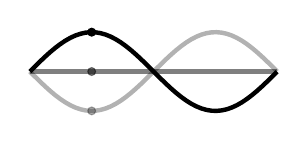
\begin{tikzpicture}[scale=0.5]

\draw [ultra thick,domain=0:2*3.14, samples=50] plot (\x, {+sin(\x r)});
\draw [ultra thick,domain=0:2*3.14, samples=50,opacity=0.5] plot (\x, {0});
\draw [ultra thick,domain=0:2*3.14, samples=50,opacity=0.3] plot (\x, {-sin(\x r)});

\draw[fill=black] (3.14*0.5,1,0) circle (0.1 );
\draw[fill=black,opacity=0.5] (3.14*0.5,0,0) circle (0.1 );
\draw[fill=black,,opacity=0.3] (3.14*0.5,-1,0) circle (0.1 );
 \end{tikzpicture}
 \begin{itemize}
 \item Material Point moves along with spatial point
 \item Used for solids
 \end{itemize}
\end{block}

\column{0.3\textwidth}
\begin{block}{Eulerian}


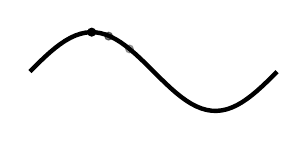
\begin{tikzpicture}[scale=0.5]

\draw [ultra thick,domain=0:2*3.14, samples=50] plot (\x, {3+sin(\x r)});
%\draw [ultra thick,domain=0:2*3.14, samples=50,opacity=0.7] plot (\x, {0});
%\draw [ultra thick,domain=0:2*3.14, samples=50,opacity=0.3] plot (\x, {-sin(\x r)});

\draw[fill=black] (3.14*0.5,3+1,0) circle (0.1 );
\draw[fill=black,opacity=0.5] (2,3+0.9,0) circle (0.1 );
\draw[fill=black,,opacity=0.3] (2.53,3+0.574,0) circle (0.1 );



 \end{tikzpicture}
 \begin{itemize}
 \item Material Point moves but spatial point stays
 \item Used for fluids
 \end{itemize}
 
 \end{block}
\column{0.3\textwidth}
\begin{block}{Mixed}


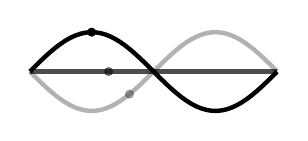
\begin{tikzpicture}[scale=0.5]


\draw [ultra thick,domain=0:2*3.14, samples=50] plot (\x, {-3+sin(\x r)});
\draw [ultra thick,domain=0:2*3.14, samples=50,opacity=0.7] plot (\x, {-3});
\draw [ultra thick,domain=0:2*3.14, samples=50,opacity=0.3] plot (\x, {-3-sin(\x r)});

\draw[fill=black] (3.14*0.5,-3+1,0) circle (0.1 );
\draw[fill=black,opacity=0.5] (2,-3,0) circle (0.1 );
\draw[fill=black,,opacity=0.3] (2.53,-3-0.574,0) circle (0.1 );

 \end{tikzpicture}
 \begin{itemize}
 \item Both point moves independently.
 \item Moving Material
 \end{itemize}
 
 \end{block}
 
\end{columns}
\begin{block}{Material Derivative}


\begin{equation*}
\frac{d(\circ)}{dt}=\frac{\partial(\circ)}{\partial t} + V_i \cdot (\circ)_{,i} 
\end{equation*}
\begin{equation*}
  v_i = \dot{u_i}+V_1u_{i,1}
\end{equation*} 

\end{block}

\end{frame}


\end{comment}


\begin{frame}
%\frametitle{Variation of the kinetic energy}
First the integration along thickness is done
\begin{equation*}
\int_{-\frac{h}{2}}^{\frac{h}{2}} \mathbf{v}^T\rho\mathbf{v} dz =
\int_{-\frac{h}{2}}^{\frac{h}{2}}
\left(
\rho\dot{u_i}\dot{u_i}
+
2 \rho V_1 \dot{u_i} u_{i,1}
+
\rho V_1^2 u_{i,1} u_{i,1}
\right) dz
\end{equation*}
\begin{equation*}
 =
\rho \dot{\tilde{u_i}} Z_{ij} \dot{\tilde{u_i}}
+
2 \rho V_1 \dot{\tilde{u_i}} Z_{ij} \tilde{u}_{j,1} 
+
\rho V_1^2 \tilde{u}_{j,1} Z_{ij} \tilde{u}_{j,1}
\end{equation*}
substituting it in the kinetic energy equation
\begin{equation*}
T = \frac{1}{2} \int \int_\Omega \left(
\rho \dot{\tilde{u_i}} Z_{ij} \dot{\tilde{u_i}}
+
\rho V_1 \dot{\tilde{u_i}} Z_{ij} \tilde{u}_{j,1} 
+
\rho V_1^2 \tilde{u}_{j,1} Z_{ij} \tilde{u}_{j,1}
 \right) d\Omega
\end{equation*}
\begin{columns}
\column{0.7\textwidth}
\begin{block}{Variations of Kinetic Energy}


\begin{equation*}
\begin{split}
\delta T = & \int \int_\Omega 
\rho \dot{\tilde{u_i}} Z_{ij} \delta \dot{\tilde{u_i}}
+
\rho V_1 \delta \dot{\tilde{u_i}} Z_{ij} \tilde{u}_{j,1} \\ &
  +  
\rho V_1  \dot{\tilde{u_i}} Z_{ij} \delta \tilde{u}_{j,1} 
+
\rho V_1^2 \tilde{u}_{j,1} Z_{ij} \delta \tilde{u}_{j,1}
 d\Omega
\end{split}
\end{equation*}

\end{block}

\column{0.3\textwidth}
\begin{equation*}
Z_{ij}=
\begin{bmatrix}
\frac{h^3}{12} & 0 & 0 \\
0 & \frac{h^3}{12} &  0 \\
0 &   0 & h 
\end{bmatrix}
\end{equation*}
\end{columns}

\end{frame}



\subsection{External Work}
\begin{frame}
\frametitle{External Work}
more summation and write them separately for variations. 
\begin{equation*}
 W=\sum_i^{nb} W_i=\sum_i^{nb} \int_{\Omega_i} q_i \mathbf{ u_i}  d \Omega_i
\end{equation*}

\begin{block}{Variation of the external work}
\begin{equation*}
\delta W=\sum_i^{nb} \int_{\Omega_i} q_i \mathbf{\delta u_i}  d \Omega_i
\end{equation*}
\end{block}



\end{frame}


\begin{frame}
\frametitle{The Weak form} 
Substituting Everything in Hamilton principle gives
\begin{equation*}
\begin{split}
 \int_{t_0}^{t_1} \left( \delta T - \delta V + \delta W \right) dt    =  0 
\end{split} 
\end{equation*}
Using integration by parts the following equation is  obtained. First term will vanish as the variation of displacement at beginning and end time is zero.  
\begin{equation*}
\begin{split}
 \int \int_\Omega 
+
\rho \dot{\tilde{u_i}} Z_{ij} \delta \tilde{u_i}
+
\rho V_1 \delta {\tilde{u_i}} Z_{ij} \tilde{u}_{j,1} 
+  
\rho V_1 {\tilde{u_i}} Z_{ij} \delta \tilde{u}_{j,1}  
 d \Omega  \Big|_{t_0}^{t_1} 
 \\ +
 \int_{t_0}^{t_1} \int \int_\Omega 
-
\rho \ddot{\tilde{u_i}} Z_{ij} \delta {\tilde{u_i}}
-
\rho V_1 \delta {\tilde{u_i}} Z_{ij} \dot{\tilde{u}}_{j,1} 
-  
\rho V_1  \tilde{u_i} Z_{ij} \delta \dot{\tilde{u}}_{j,1} 
+
\rho V_1^2 \tilde{u}_{j,1} Z_{ij} \delta \tilde{u}_{j,1}
\\ 
- 
\kappa^T \tilde{D} \delta\kappa 
-
\left(\epsilon^S\right)^T \tilde{D_c} \delta\epsilon^S 
- 
 w_{, \alpha} \tilde{\sigma}^A  \delta w_{, \alpha}  d \Omega     
 +   
 \sum_i^{nb}   \int  \int_{\Omega_i} q_i \mathbf{\delta u_i}  d \Omega_i dt = 0
\end{split} 
\end{equation*}
$
\int_{t_0}^{t_1} \chi dt = 0
$
For this to be true
$
 \chi  = 0
$  must also be true . Final Weak Form is 
\begin{equation*}
\begin{split}
 \int \int_\Omega 
\rho \ddot{\tilde{u_i}} Z_{ij} \delta {\tilde{u_i}}
+
2 \rho V_1 \delta {\tilde{u_i}} Z_{ij} \dot{\tilde{u}}_{j,1} 
-
\rho V_1^2 \tilde{u}_{j,1} Z_{ij} \delta \tilde{u}_{j,1}
\\ 
+
\kappa^T \tilde{D} \delta\kappa 
+
\left(\epsilon^S\right)^T \tilde{D_c} \delta\epsilon^S 
+ 
 w_{, \alpha} \tilde{\sigma}^A  \delta w_{, \alpha} d \Omega     
=  
 \sum_i^{nb}   \int  \int_{\Omega_i} q_i \mathbf{\delta u_i}  d \Omega_i dt
\end{split} 
\end{equation*}


\end{frame}


\begin{frame}
\frametitle{Strong Form}
\begin{block}{The weak form}
\begin{equation*}
\begin{split}
 \int \int_\Omega 
\rho \ddot{\tilde{u_i}} Z_{ij} \delta {\tilde{u_i}}
+
2 \rho V_1 \delta {\tilde{u_i}} Z_{ij} \dot{\tilde{u}}_{j,1} 
-
\rho V_1^2 \tilde{u}_{j,1} Z_{ij} \delta \tilde{u}_{j,1}
\\ 
+
\kappa^T \tilde{D} \delta\kappa 
+
\left(\epsilon^S\right)^T \tilde{D_c} \delta\epsilon^S 
+ 
 w_{, \alpha} \tilde{\sigma}^A  \delta w_{, \alpha} d \Omega     
=  
 \sum_i^{nb}   \int  \int_{\Omega_i} q_i \mathbf{\delta u_i}  d \Omega_i dt
\end{split} 
\end{equation*}

\end{block}

$
\int \int_\Omega \chi d\Omega = 0
$
For this to be true
$
 \chi  = 0
$  must also be true and by considering $\epsilon^S=0$, $\tilde{\sigma}^A=N_x$ and $\tilde{u}_1 =\tilde{u}_2 = 0 $ we get the strong  form. 
Only single force is considered, which is $nb=1$, $q_i=F$ and $\Omega_i = \Omega$
\begin{block}{Final strong Form}

\begin{equation*}
\begin{split}
\rho h \left( \frac{\partial ^ 2 w}{\partial t ^ 2 }+2V_1\frac{\partial ^ 2 w}{\partial x \partial t}-V_1^2
\frac{\partial ^ 2 w}{\partial x ^ 2 } \right)  + D  \triangledown ^4 w+ N_xh\frac{\partial ^ 2 w}{\partial x ^ 2 }=F 
\end{split} 
\end{equation*}


\end{block}
\begin{equation*}
\triangledown ^4 w = \frac{\partial ^ 4 w}{\partial x ^ 4 }+2 \frac{\partial ^ 4 w}{\partial x ^ 2 \partial y ^ 2 } + \frac{\partial ^ 4 w}{\partial Y ^ 4 } \qquad D = \frac{Eh^3}{12 \left( 1 - \nu^2 \right) }
\end{equation*}
\end{frame}

\section{Finite Element Formulation}


\begin{frame}
\frametitle{Finite Element Method}
In Finite element a  continuous domain is discretized into elements. Each elements are connect by nodes.   
\begin{figure}[h!]
\centering
\minipage{0.8\textwidth}%
  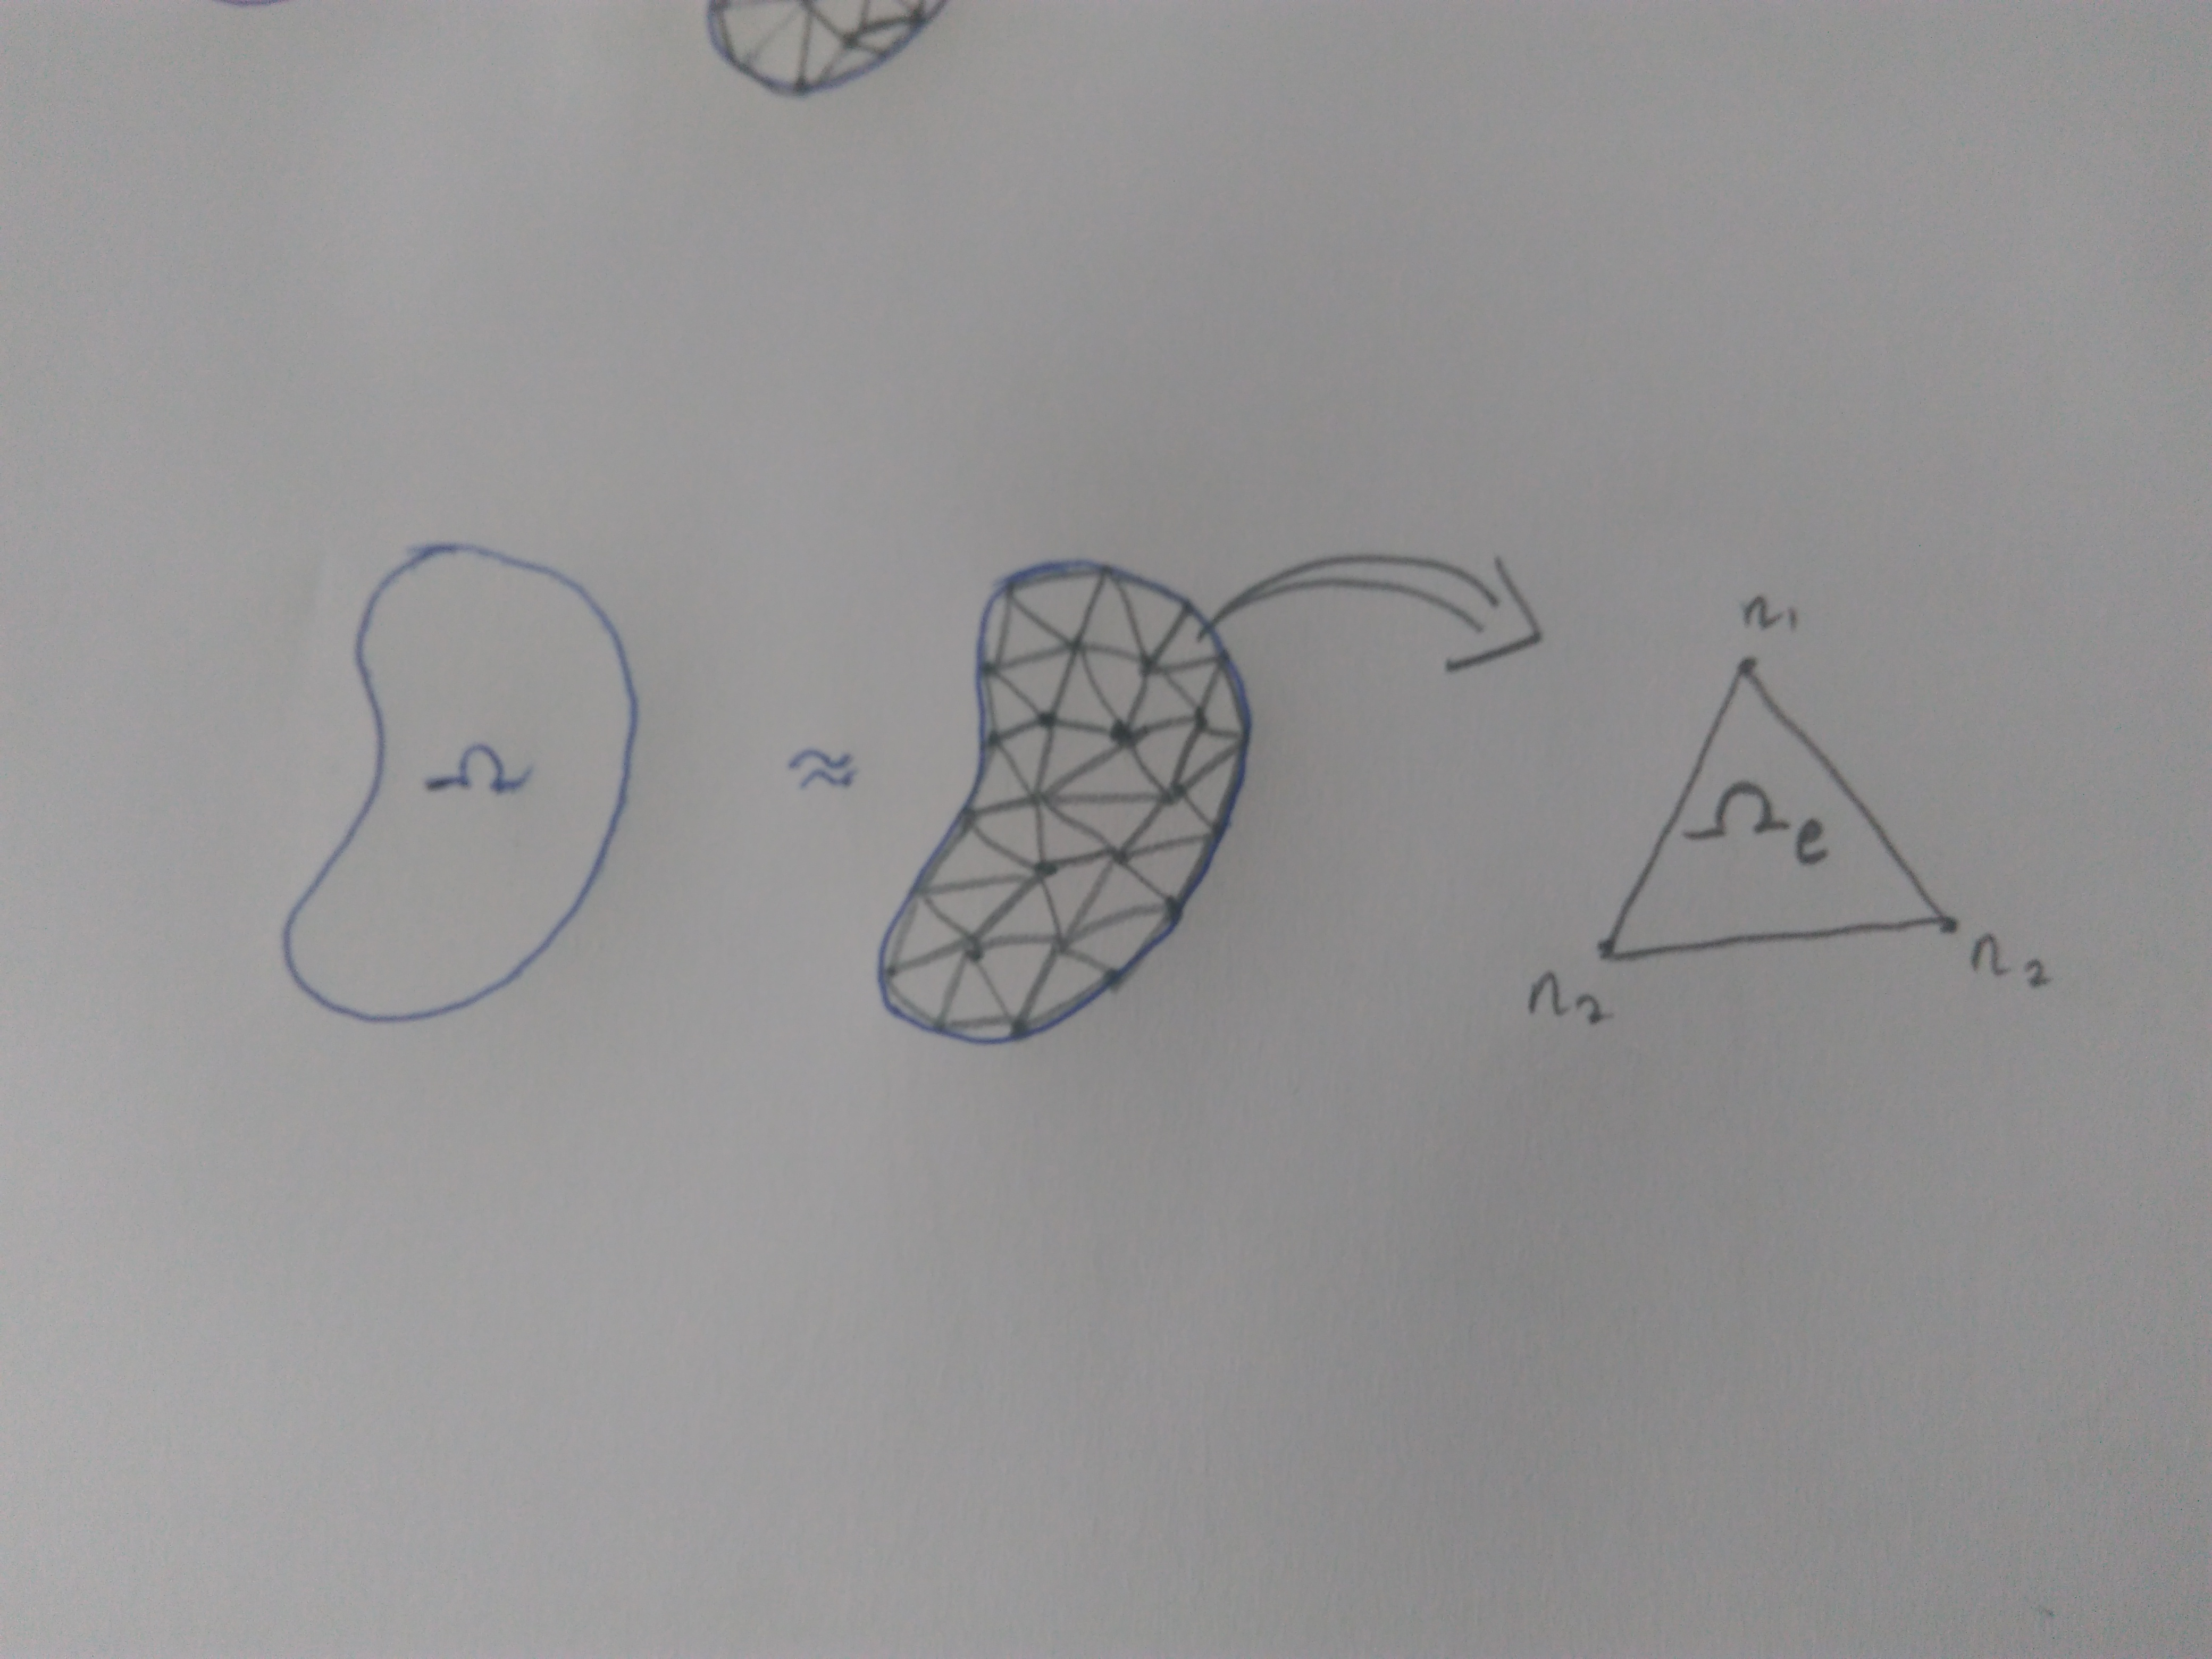
\includegraphics[width=\linewidth,trim={10cm 30cm 8cm 30cm},clip]{FEM.jpg}
  % \caption{FEM solution plot}
\endminipage
\end{figure} 
\begin{equation*}
\Omega \approx \sum_{i}^{nE} \Omega_e^i
\end{equation*}
The displacement is represented as a degree of freedom of the system.
\begin{equation*}
\tilde{u} = \left[ w, \theta_x , \theta_y  \right]^T \quad \theta_x=\frac{\partial w}{\partial x} \quad \theta_y=\frac{\partial w}{\partial y}
\end{equation*}
\end{frame}

\begin{frame}
\frametitle{Shape function of a rectangular  element}
The displacement field over the element is given as the sum of product of shape function and nodal displacements. here $nN$ is the total number of nodes in a element
 \begin{columns}
 \column{0.5\textwidth}
\begin{equation*}
\tilde{\mathbf{u}} \approx \sum_{i=1}^{nN}\left(N_iw_i+\overline{N}_i\theta_{x_i}+\overline{\overline{N}}_i\theta_{y_i}\right)
\end{equation*}
\begin{align*}
N_1= \frac{1}{4ab}\left(1-x\right) \left(1-y\right)\\
{N}_2 = \frac{1}{4ab}\left(1+x\right) \left(1-y\right)\\
{N}_4= \frac{1}{4ab}\left(1-x\right) \left(1+y\right)\\
N_3=  \frac{1}{4ab}\left(1-x\right) \left(1-y\right)
\end{align*}
For Ressiner Mindlin  element
\begin{equation*}
N_i =\overline{N}_i =\overline{\overline{N}}_i
\end{equation*}

 \column{0.5\textwidth}
\begin{figure}[h!]
\centering
\subfile{shapefun.tex}
%\caption{NAS277} \label{NAS277sch}
\end{figure}
\end{columns}
\end{frame}





\begin{frame}
\frametitle{Representation of Displacements and Strains in terms of Shape Function.}
The FE approximation 
\begin{equation*}
\tilde{\mathbf{u}} \approx \sum_{i=1}^{nN}\left(N_iw_i+\overline{N}_i\theta_{x_i}+\overline{\overline{N}}_i\theta_{y_i}\right)
\end{equation*}
is written in matrix format as
\begin{equation*}
\tilde{\mathbf{u}} \approx 
\begin{bmatrix}
N_1 & 0 & 0  & \cdots & N_{nN} & 0 & 0 \\
0 & \overline{N}_1 & 0  & \cdots & 0 & \overline{N}_{nN} & 0 \\
0 & 0 & \overline{\overline{N}}_1 & \cdots & 0 & 0 & \overline{\overline{N}}_{nN} \\
\end{bmatrix}
\left\{
\begin{array}{r}
w_1 \\
\theta_{x_1} \\
\theta_{y_1} \\
\vdots \\
w_{nN} \\
\theta_{x_{nN}} \\
\theta_{y_{nN}} \\
\end{array} \right\}
=
\mathbf{N} \tilde{\mathbf{u}}^e 
\end{equation*}
similarly for the velocity and acceleration as they are independent of time.
\begin{equation}
\dot{\tilde{ \mathbf{ u}} } \approx \mathbf{N}  \dot{\tilde{\mathbf{u}}}^e
 \qquad  
\ddot{\tilde{ \mathbf{ u}} } \approx \mathbf{N}  \ddot{\tilde{\mathbf{u}}}^e
\end{equation}
\end{frame}

\begin{frame}
\frametitle{Representation of Strains in terms of Shape Function.}
The Bending strain $\kappa = \triangle \tilde{\mathbf{u}} $ as FE matrix is given below. We can see that first column goes to zero since the double derivative shape function is zero.
\begin{equation*}
\mathbf{ \kappa } \approx 
\begin{bmatrix}
0 & \overline{N}_{1,1} & 0 & \cdots & 0 \\
0&  0 & \overline{\overline{N}}_{1,2}  & \cdots & \overline{\overline{N}}_{nN,2} 
\\
0&  \overline{N}_{1,2} & \overline{\overline{N}}_{1,1}  & \cdots & \overline{\overline{N}}_{nN,1} 
\end{bmatrix} 
\left\{
\begin{array}{r}
w_1 \\
\theta_{x_1} \\
\theta_{y_1} \\
\vdots \\
\theta_{y_{Nn}} \\
\end{array} \right\}=\mathbf{ B } \tilde{\mathbf{u}}^e
\end{equation*}
similarly for the shear strain is represented as
\begin{equation}
\tilde{\mathbf{\epsilon}}^S \approx 
\begin{bmatrix}
N_{1,1} & \overline{N}_{1} & 0 & \cdots & 0 
\\
N_{1,2} & 0 & \overline{\overline{N}}_{1} & \cdots & \overline{\overline{N}}_{nN} 
\end{bmatrix} 
\left\{
\begin{array}{r}
w_1 \\
\theta_{x_1} \\
\theta_{y_1} \\
\vdots \\
\theta_{y_{Nn}} \\
\end{array} \right\}=\mathbf{ B_S }\tilde{\mathbf{u}}^e
\end{equation}
$N_{1,2}$ represent $\dfrac{dN_1}{dy} $. $N_1$ is the shape function of w displacement in first node.
\end{frame}


\begin{frame}

\begin{equation*}
\tilde{u}_{1, \alpha} \approx 
\begin{bmatrix}
{N}_{1,1} & 0 & 0 &{N}_{2,1} & \cdots & 0 \\
{N}_{1,2} & 0 & 0 &{N}_{2,2} & \cdots & 0 \\ 
\end{bmatrix} 
\left\{
\begin{array}{r}
w_1 \\
\theta_{x_1} \\
\theta_{y_1} \\
w_{2} \\
\vdots \\
\theta_{y_{nN}} \\
\end{array} \right\}=\mathbf{ H_A }\tilde{\mathbf{u}}^e
\end{equation*}

\begin{equation*}
\tilde{u}_{\alpha, 1} \approx 
\begin{bmatrix}
{N}_{1,1} & 0 & 0 & \cdots & 0 \\
0 & \overline{N}_{2,1} & 0 & \cdots & 0 \\ 
0 & 0 & \overline{\overline{N}}_{3,1} & \cdots & \overline{\overline{N}}_{3,3} \\ 
\end{bmatrix} 
\left\{
\begin{array}{r}
w_1 \\
\theta_{x_1} \\
\theta_{y_1} \\
\vdots \\
\theta_{y_{nN}} \\
\end{array} \right\}=\mathbf{ H_v }\tilde{\mathbf{u}}^e
\end{equation*}



The FE approx for the body force is given as
\begin{equation*}
\tilde{w} \approx 
\begin{bmatrix}
{N}_{1} & 0 & 0 &{N}_{2} &\cdots & 0 
\end{bmatrix} 
\left\{
\begin{array}{r}
w_1 \\
\theta_{x_1} \\
\theta_{y_1} \\
w_2 \\
\vdots \\
\theta_{y_{nN}} \\
\end{array} \right\}=\mathbf{ N_f }\tilde{\mathbf{u}}^e
\end{equation*}
\end{frame}



\begin{frame}
\frametitle{Weak Form to FE format}
The Finite Element Matrix equation is given as

\begin{equation*}
\begin{split} 
\int \int_\Omega 
\left(
\rho
\left[ \mathbf{N}  \right]
\left[ \mathbf{Z}  \right]
\left[ \mathbf{N}  \right] 
\{ \ddot{\tilde{\mathbf{u}}}^e \}
\right) 
\delta \tilde{\mathbf{u}}^e
+
\left( 
2 \rho V_1
\left[ \mathbf{N}  \right]
\left[ \mathbf{Z}  \right]
\left[ \mathbf{H_v}  \right] 
\{ \dot{\tilde{\mathbf{u}}}^e \}
\right) 
\delta \tilde{\mathbf{u}}^e \\
-
\left( 
 \rho V_1^2
\left[ \mathbf{H_v}  \right]
\left[ \mathbf{Z}  \right]
\left[ \mathbf{H_v}  \right] 
\{\tilde{\mathbf{u}}^e \}
\right) 
\delta \tilde{\mathbf{u}}^e  
+
\left( 
\left[ \mathbf{B}  \right]
\left[ \mathbf{\tilde{D}}  \right]
\left[ \mathbf{B}  \right] 
\{\tilde{\mathbf{u}}^e \}
\right) 
\delta \tilde{\mathbf{u}}^e  \\
+
\left( 
\left[ \mathbf{B_S}  \right]
\left[ \mathbf{\tilde{D}_S}  \right]
\left[ \mathbf{B_S}  \right] 
\{\tilde{\mathbf{u}}^e \}
\right) 
\delta \tilde{\mathbf{u}}^e
+
\left( 
\left[ \mathbf{H_A}  \right]
\left[ \mathbf{\tilde{N}_A}  \right]
\left[ \mathbf{H_A}  \right] 
\{\tilde{\mathbf{u}}^e \}
\right) 
\delta \tilde{\mathbf{u}}^e
d \Omega
   \\
 =   
 \sum_i^{nb}   \int  \int_{\Omega_i} 
\left(  
 q_i 
\left[ \mathbf{\tilde{N}_f}  \right] 
\right)  
\delta \tilde{\mathbf{u}}^e
  d \Omega_i  
\end{split} 
\end{equation*}

\end{frame}

\begin{frame}
\frametitle{FEM matrices}
After rearranging them to their respective groups we get.
\begin{equation*}
\left[ \mathbf{M}^e  \right] 
\{ \ddot{\mathbf{u}}^e \}
+
\left[ \mathbf{C}  \right] 
\{ \dot{\mathbf{u}}^e \}
+
\left[ \mathbf{K}^e  \right] 
\{\mathbf{u}^e \}
=
\{ \mathbf{F}^e \}
\end{equation*}
where 
\begin{align*}
&\left[ \mathbf{M}^e  \right]  
= \rho
\int \int_\Omega 
\left(
\left[ \mathbf{N}  \right]
\left[ \mathbf{Z}  \right]
\left[ \mathbf{N}  \right] 
\right)  d \Omega  \\
&\left[ \mathbf{C}^e  \right]   
= 2 \rho V_1
\int \int_\Omega 
\left( 
\left[ \mathbf{N}  \right]
\left[ \mathbf{Z}  \right]
\left[ \mathbf{H_v}  \right] 
\right)  d \Omega  \\ &
\left[ \mathbf{K} ^e \right] 
=  - \rho V_1^2
\int \int_\Omega 
\left( 
\left[ \mathbf{H_v}  \right]
\left[ \mathbf{Z}  \right]
\left[ \mathbf{H_v}  \right] 
\right)  d \Omega + 
\int \int_\Omega  
\left[ \mathbf{B}  \right]
\left[ \mathbf{\tilde{D}}  \right]
\left[ \mathbf{B}  \right]  
  d \Omega   \\  &  \quad +
  \int \int_\Omega  
\left[ \mathbf{B_S}  \right]
\left[ \mathbf{\tilde{D}_S}  \right]
\left[ \mathbf{B_S}  \right] 
  d \Omega +
  \int \int_\Omega  
\left[ \mathbf{H_A}  \right]
\left[ \mathbf{\tilde{N}_A}  \right]
\left[ \mathbf{H_A}  \right]  
  d \Omega  \\ &
\{ \mathbf{F}^e \}  = 
 \sum_i^{nb}   \int  \int_{\Omega_i}   
 q_i 
\left[ \mathbf{\tilde{N}_f}  \right] 
  d \Omega_i    
\end{align*}
\end{frame}


\begin{frame}
\frametitle{Gauss Quadrature}
Gauss Quadrature is used for numerical integration over the element.
\begin{columns}
\column{0.5\textwidth}
\begin{figure}[h!]
\centering
\subfile{gauss.tex}
%\caption{NAS277} \label{NAS277sch}
\end{figure}
\column{0.5\textwidth}
\begin{equation*}
\begin{split}
\int \int f(x,y) dx dy = \\
 \sum_{i = 1}^{nx} \sum_{j = 1}^{ny} w_i  w_j \cdot f(ix,jy) 
\end{split}
\end{equation*}
\begin{equation*}
\begin{split}
w_i = w_j =1
\end{split}
\end{equation*}
$w_i$ and $w_j$ are the Gauss weight.\\
 $ix$ and $jy$ are the Gauss Points. 

\end{columns}

\end{frame}


\begin{frame}
\frametitle{Iso parametric Shape Function}
\begin{figure}[h!]
\centering
\subfile{iso.tex}
%\caption{NAS277} \label{NAS277sch}
\end{figure}
\begin{equation*}
\begin{split}
N_1 =\frac{1}{4}\left(1-\xi \right)\left( 1-\eta \right)\quad  & N_2=\frac{1}{4}\left(1+\xi \right)\left( 1-\eta \right) \\
 N_4 =\frac{1}{4}\left(1-\xi \right)\left(1+ \eta \right)\quad  & N_3 =\frac{1}{4}\left(1+\xi \right)\left( 1+\eta \right)
\end{split}
\end{equation*}


\end{frame}
\begin{frame}
\frametitle{Jacobian Transformation}
Derivation of the shape function by the coordinated in parent element using chain rule gives us
\begin{equation*}
\dfrac{\partial N }{ \partial \xi } = 
\dfrac{\partial N }{ \partial x }
\dfrac{ \partial x }{\partial \xi }  
+
\dfrac{\partial N }{ \partial y }
\dfrac{ \partial y }{\partial \xi } 
\end{equation*}
This relation is written in matrix format which gives us J matrix or jacobian matrix. 
\begin{equation*}
\left\{
\begin{array}{r}
\dfrac{\partial N }{ \partial \xi }  \\
\dfrac{\partial N }{ \partial \eta }  \\
\end{array}
\right\}
=
\begin{bmatrix}
\dfrac{ \partial x }{\partial \xi }   &
\dfrac{ \partial y }{\partial \xi } \\
\dfrac{ \partial x }{\partial \eta }   &
\dfrac{ \partial y }{\partial \eta } \\
\end{bmatrix}
\left\{
\begin{array}{r}
\dfrac{\partial N }{ \partial x }  \\
\dfrac{\partial N }{ \partial y }  \\
\end{array}
\right\}
\quad
J=\begin{bmatrix}
\dfrac{ \partial x }{\partial \xi }   &
\dfrac{ \partial y }{\partial \xi } \\
\dfrac{ \partial x }{\partial \eta }   &
\dfrac{ \partial y }{\partial \eta } \\
\end{bmatrix}
\end{equation*}
det(J) must always be greater than zero. det(J) = 0  means the 2D element disappears into 1D. Jacobian is also a important measure of quality of the mesh.
\begin{equation*}
\left\{
\begin{array}{r}
\dfrac{\partial N }{ \partial x }  \\
\dfrac{\partial N }{ \partial y }  \\
\end{array}
\right\}
=
J^{-1}
\left\{
\begin{array}{r}
\dfrac{\partial N }{ \partial \xi }  \\
\dfrac{\partial N }{ \partial \eta }  \\
\end{array}
\right\}
\end{equation*}
The Inverse relation is employed to find the derivative of shape function from parent element.
\end{frame}

\begin{frame}
\frametitle{Final FEA matrix}
\begin{equation*}
\left[ \mathbf{M^e}  \right] 
=
\sum_{i = 1}^{ng}
\rho\left(w_i
\left[ \mathbf{N(i)}  \right]^T
\left[ \mathbf{Z}  \right]
\left[ \mathbf{N(i)}  \right] 
det(J)\right)  d \Omega
\end{equation*}
All the Element mass Matrices $\left[ \mathbf{M^e}  \right]$ are assembled in the final Mass Matrix $\left[ \mathbf{M} \right]$. Which gives us the  ODE in terms of FE matrices.

\begin{equation*}
\left[ \mathbf{M}  \right] 
\{ \ddot{\mathbf{u}} \}
+
\left[ \mathbf{C}  \right] 
\{ \dot{\mathbf{u}} \}
+
\left[ \mathbf{K}  \right] 
\{\mathbf{u} \}
=
\{ \mathbf{F} \}
\end{equation*}
\end{frame}


\begin{frame}
\frametitle{Solution Procedure}
\textbf{Static Analysis:}\\

To solve a static system  
\begin{equation*}
 \left[ \mathbf{K}  \right] 
\{\mathbf{u} \}
=
\{ \mathbf{F} \} 
\end{equation*}
 $ u=K \backslash F $ command is used since $u=K^{-1}F$ is a very expensive task. $u=K \backslash F$ command first factorizes the K matrix into upper and lower triangle then solves the system which is a much more efficient process.
\\
\textbf{Modal Analysis:}\\


\begin{equation*}
\mathbf{M}\mathbf{\ddot{{ u}}}+\mathbf{K}\mathbf{{ u}}=0
\end{equation*}
is converted in to a eigenvalue  problem
\begin{equation*}
\left( \mathbf{K} - \omega^2 \mathbf{M}  \right) \overline{\mathbf{u} } = 0 \qquad { \mathbf{u}}=\overline{ \mathbf{u}}e^{i\omega t}
\end{equation*}
$\omega$ is the natural frequency and $\overline{\mathbf{u}}$ is the natural mode. In MATLAB, [V,D]=eig(K,M) function is used to do the modal analysis.
\end{frame}

\begin{frame}
\textbf{Dynamic Analysis:}\\
To solve the dynamic system
\begin{equation*}
\left[ \mathbf{M}  \right] 
\{ \ddot{\mathbf{u}} \}
+
\left[ \mathbf{C}  \right] 
\{ \dot{\mathbf{u}} \}
+
\left[ \mathbf{K}  \right] 
\{\mathbf{u} \}
=
\{ \mathbf{F} \}
\end{equation*}
Newmark time integration scheme is employed. 
\begin{block}{Newmark algorithm}
\begin{equation*}
R=F_t + \mathbf{M} \left(a_0 u_{t}+a_2 \dot{u}_{t} + a_3 \ddot{u}_{t} \right) + \mathbf{C} \left(a_1 u_{t}+a_4 \dot{u}_{t} + a_5 \ddot{u}_{t} \right) 
\end{equation*}
\begin{align*}
u_{t+1} & =\left[a_0 \mathbf{M} + a_1 \mathbf{C} + \mathbf{K} \right] ^ {-1} R \\
\dot{u}_{t+1} & =a_1 \left( u_{t+1} - u_{t} \right) - a_4 \dot{u}_t -a_5 \ddot{u}_t \\
\ddot{u}_{t+1} & =a_0 \left( u_{t+1} - u_{t}\right) - a_2 \dot{u}_t -a_3 \ddot{u}_t
\end{align*}
\end{block}
\begin{columns}
\column{0.7\textwidth}
$a_0$ .. $a_5$ are the integration variables which depends on the Integration parameters $\theta$, $\alpha$ and time step $h$. 
$u_t$,$\dot{u}_t$ and $\ddot{u}_t$ are the displacement , velocity and acceleration of current time step. $u_{t+1}$,$\dot{u}_{t+1}$ and $\ddot{u}_{t+1}$ are the displacement , velocity and acceleration of next time step. 
\column{0.3\textwidth}
Unconditionally Stable for
\begin{align*}
\theta & \geq \frac{1}{2}  \\
\alpha & \geq \frac{1}{4}\left(\frac{1}{2}+\theta \right)^2
\end{align*}

\end{columns}
\end{frame}

\section{Verification Problems}

\begin{frame}
\frametitle{TIM69 Static Analysis , Circular Plate with Point load}

\begin{columns}
\column{0.5\textwidth}

\begin{figure}[h!]
\centering
\minipage{1\textwidth}%
  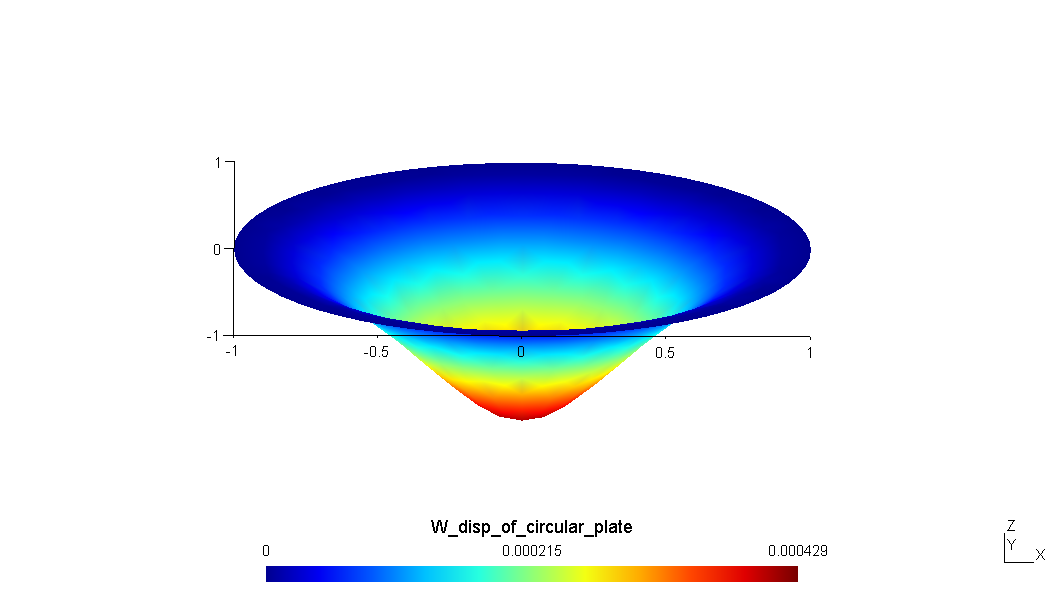
\includegraphics[width=\linewidth,trim={5cm 4cm 5cm 4cm},clip]{TIM69_pos.png}
  % \caption{FEM solution plot}
\endminipage
\end{figure}
The target analytically solution given as
\begin{equation}
w = \frac{F_z}{16 \pi D}\left[ r^2 - a^2 \right]+\frac{F_zr^2}{8 \pi D}\left[ log \frac{a}{r} \right]
\end{equation} 
 The analytical solution is -0.000434 $in$.\\ Numerical solution is $ -0.000429 in $. \\
So the Error percentage is $ 1.26 \% $. 
\column{0.5\textwidth}

\begin{table}[ht]
\renewcommand{\arraystretch}{1.5}
\centering
\begin{tabular}{ll}
\hline
\multicolumn{2}{l}{Material Property} \\ \hline  \hline
Young's Modulus ($E$)          & 5E11 $Pa$        \\
Poission's Ratio ($\nu$)       & 0.3            \\ 
    \hline
    \multicolumn{2}{l}{Geometric Data} \\ \hline  \hline
            Radius ($r$)        & 1 $m$   \\
            Thickness($t$)     &         0.01 $m$  \\
             \hline
    \multicolumn{2}{l}{Loading Data} \\ \hline  \hline
    Point Load ($F_z$)        & -1000 $N$     \\    \hline
\end{tabular}
\end{table}

\end{columns}


%\begin{table}[ht]
%\renewcommand{\arraystretch}{1.5}
%\centering
%\begin{tabular}{lll}
%\hline
%{Material } & {Geometric} & {Loading } \\ \hline  \hline
% ($E$)         = 5E11 $Pa$         & ($r$)       = 1 $m$        & ($F_z$) = -1000 $N$         \\
%($\nu$) = 0.3         &($h$)  = 0.01 $m$  &           \\ 
%            \hline
%\end{tabular}
%\end{table}

\begin{block}{Reference}
S.Timoshenko , S . Woinowsky , Theory of Plates and Shells , pg:69, Article : 19 . 
\end{block}

\end{frame}




\begin{frame}
\frametitle{VMP09 Modal Analysis , SS square Plate}

\begin{columns}
\column{0.5\textwidth}

\begin{figure}[h!]
\centering
\minipage{1\textwidth}%
  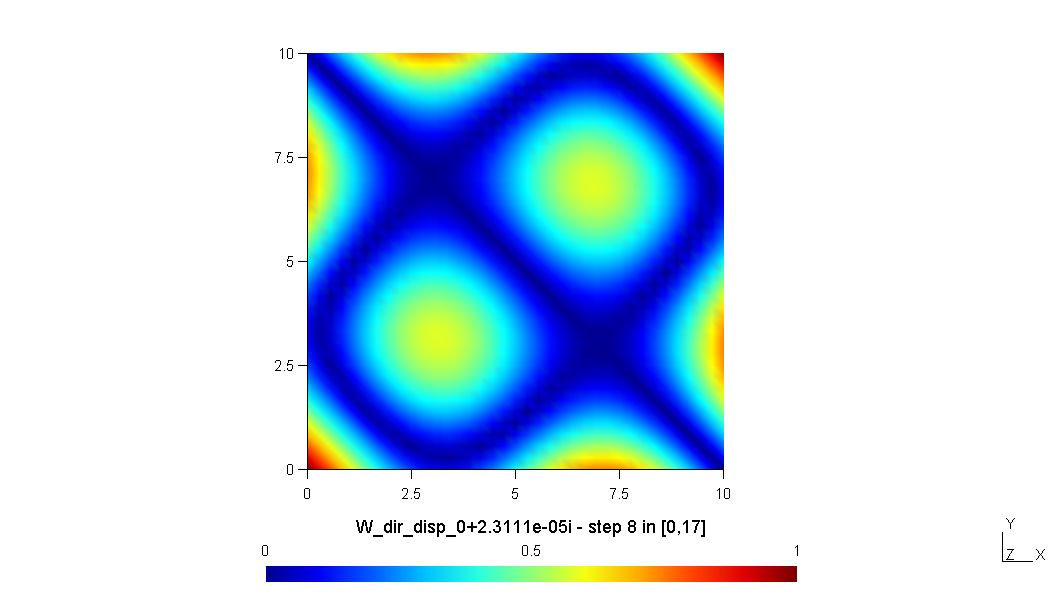
\includegraphics[width=\linewidth,trim={8cm 4cm 8cm 2cm},clip]{VMP09_T12_pos_F9.png}
  % \caption{FEM solution plot}
\endminipage
\end{figure}

The analytical frequency is 1.632 $Hz$. 
The numerical frequency is  1.626 $Hz$. \\
So the Error percentage is  0.32 $\%$ 


\column{0.5\textwidth}

\begin{table}[ht]
\renewcommand{\arraystretch}{1.5}
\centering
\begin{tabular}{ll}
\hline
\multicolumn{2}{l}{Material Property} \\ \hline  \hline
Young's Modulus ($E$)          &25E11 $Pa$        \\
Poission's Ratio ($\nu$)       & 0.3            \\ 
Density($\rho$)       &     8000         \\ 
    \hline
    \multicolumn{2}{l}{Geometric Data} \\ \hline  \hline
            length ($l$)        & 10 $m$   \\
            breath ($b$)        & 10 $m$   \\
            Thickness($t$)     &         0.01 $m$  \\
             \hline
\end{tabular}
\end{table}

\end{columns}



\begin{block}{Reference}
S.Timoshenko , S . Woinowsky , Theory of Plates and Shells , pg:69, Article : 19 . 
\end{block}

\end{frame}



\begin{comment}

\begin{frame}
\frametitle{VMP09}

\begin{figure}[h!]
\begin{subfigure}{.3\textwidth}
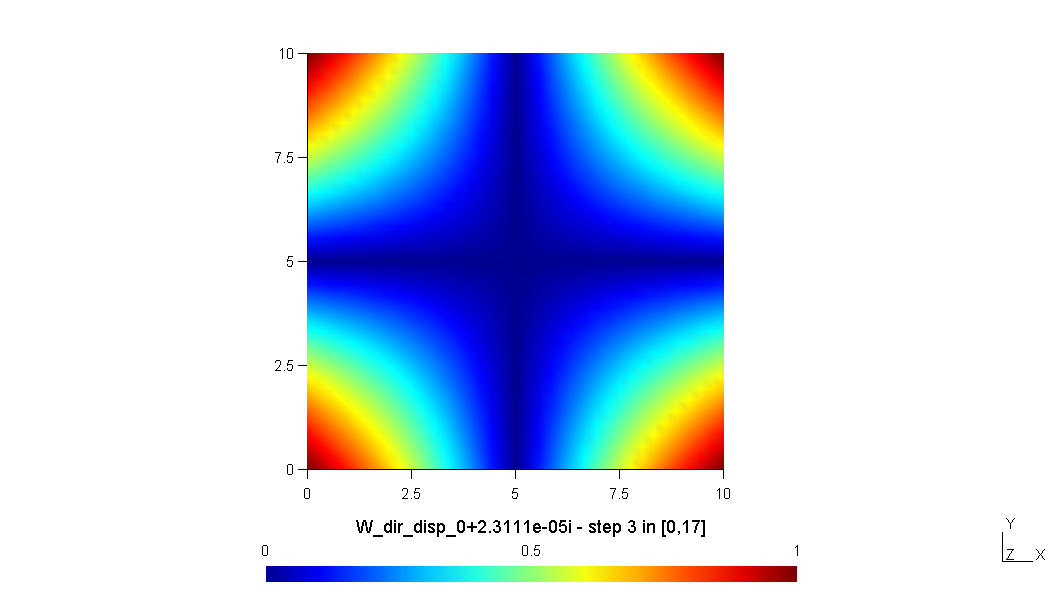
\includegraphics[width=\linewidth,trim={8cm 4cm 8cm 2cm},clip]{VMP09_T12_pos_F4.png}
%\caption{Mode Shape 4}
\end{subfigure} \hfill
\begin{subfigure}{.3\textwidth}
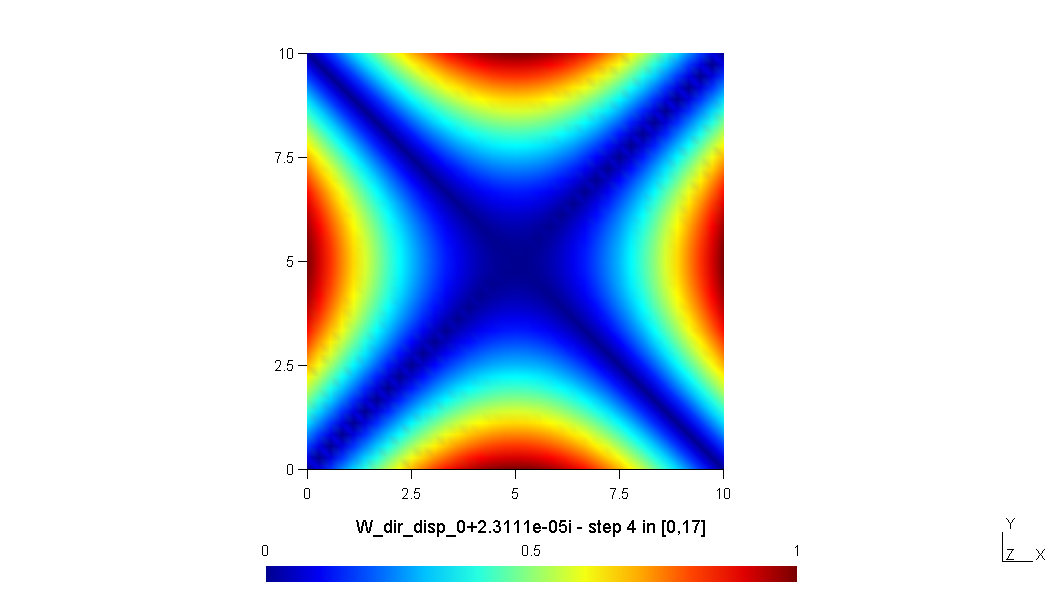
\includegraphics[width=\linewidth,trim={8cm 4cm 8cm 2cm},clip]{VMP09_T12_pos_F5.png}
%\caption{Mode Shape 5}
\end{subfigure}\hfill
\begin{subfigure}{.3\textwidth}
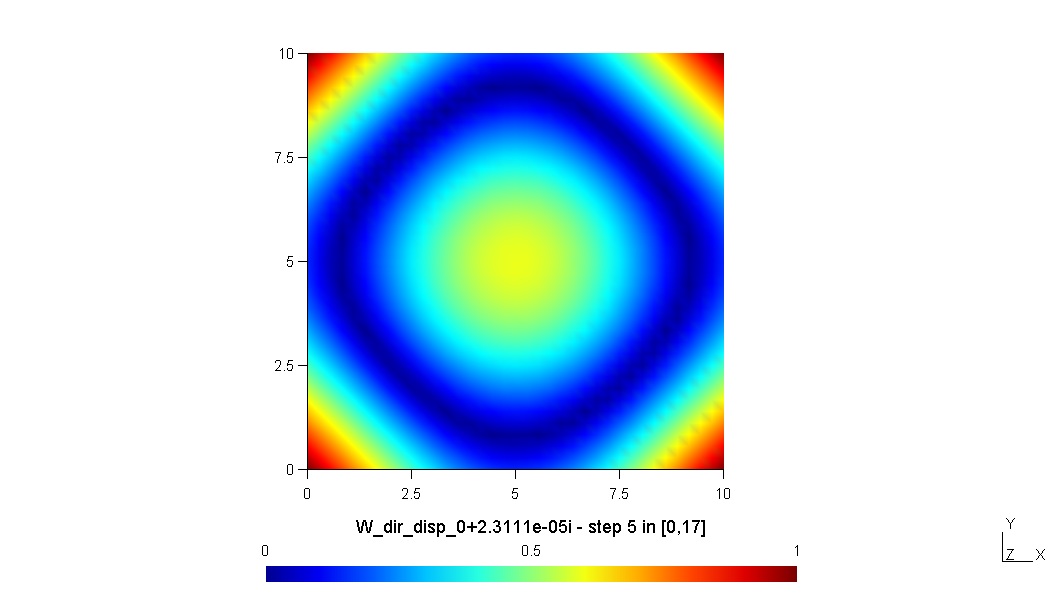
\includegraphics[width=\linewidth,trim={8cm 4cm 8cm 2cm},clip]{VMP09_T12_pos_F6.png}
%\caption{Mode Shape 6}
\end{subfigure}\vfill
\begin{subfigure}{.3\textwidth}
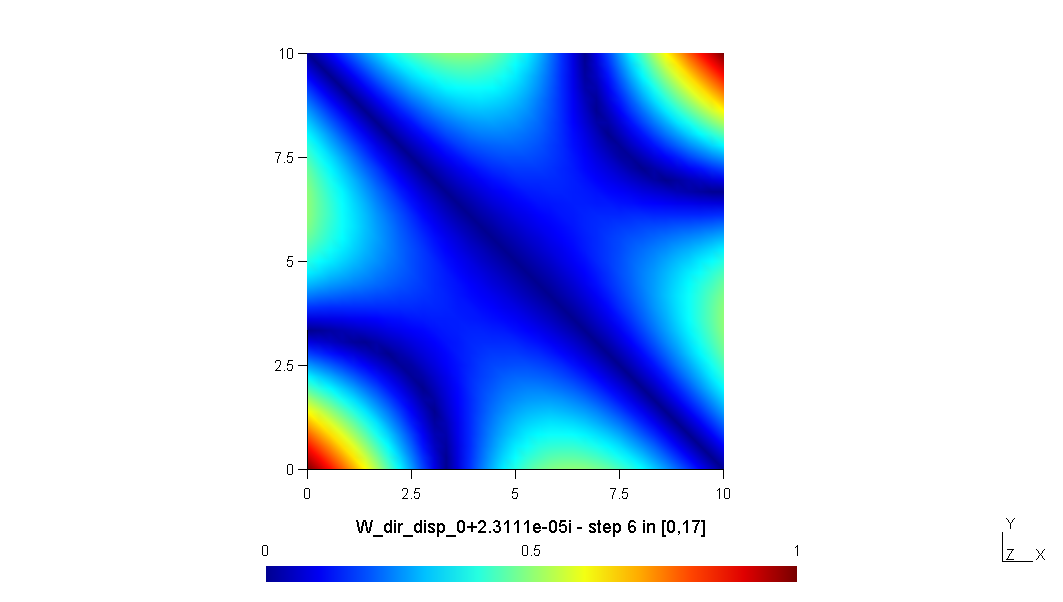
\includegraphics[width=\linewidth,trim={8cm 4cm 8cm 2cm},clip]{VMP09_T12_pos_F7.png}
%\caption{Mode Shape 7}
\end{subfigure} \hfill
\begin{subfigure}{.3\textwidth}
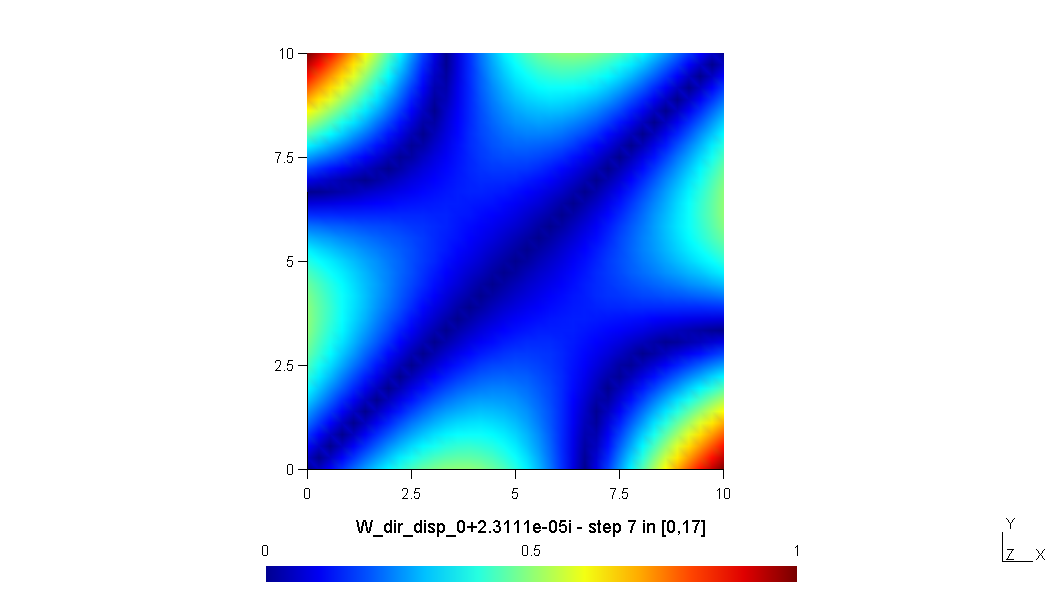
\includegraphics[width=\linewidth,trim={8cm 4cm 8cm 2cm},clip]{VMP09_T12_pos_F8.png}
%\caption{Mode Shape 8}
\end{subfigure}\hfill
\begin{subfigure}{.3\textwidth}
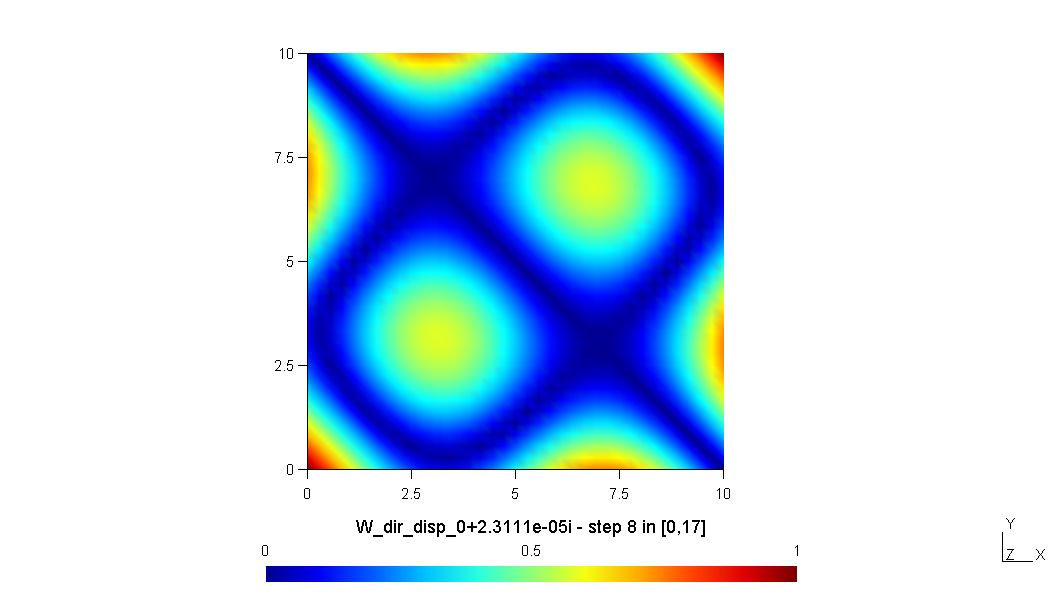
\includegraphics[width=\linewidth,trim={8cm 4cm 8cm 2cm},clip]{VMP09_T12_pos_F9.png}
%\caption{Mode Shape 9}
\end{subfigure}
%\caption{Natural Modes of a Square Plate}
\end{figure}

\begin{block}{Reference}
NAFEMS Manual. Solution Retrieved from Ansys verification problem (VMP09-T12).
\end{block}
Error $\%$ = 0.32 $\%$.



\end{frame}
\end{comment}


\begin{frame}
\frametitle{NAS227 modal analysis of thin plate with axial load}

\begin{columns}
\column{0.5\textwidth}

\begin{figure}[h!]
\centering
\begin{subfigure}{1\textwidth}
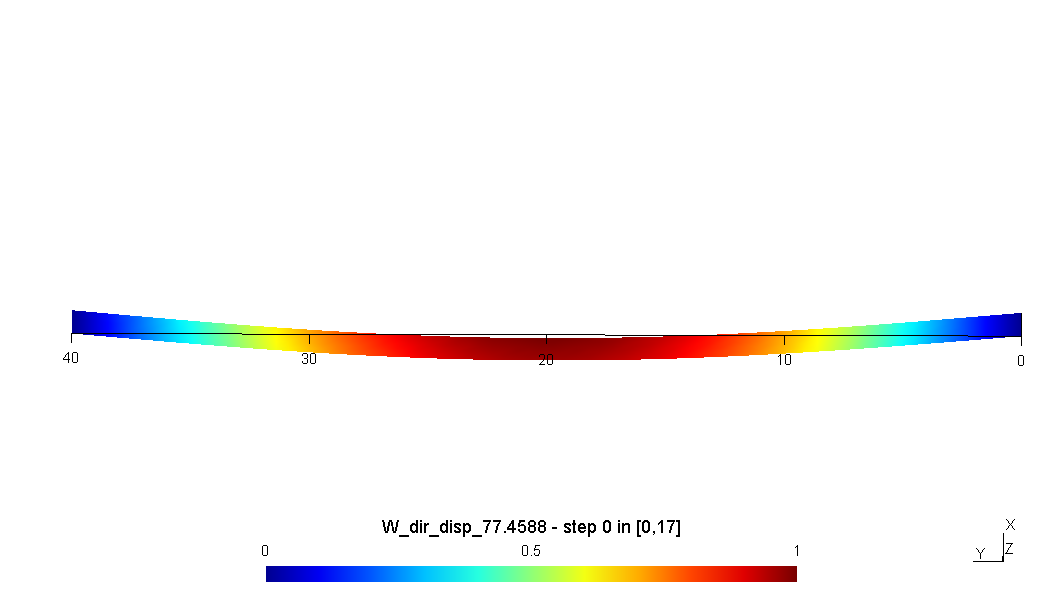
\includegraphics[width=\linewidth,trim={0 8cm 0 8cm},clip]{NAS277_pos_1.png}
%\caption{Mode Shape 1}
\end{subfigure} \vfill
\begin{subfigure}{1\textwidth}
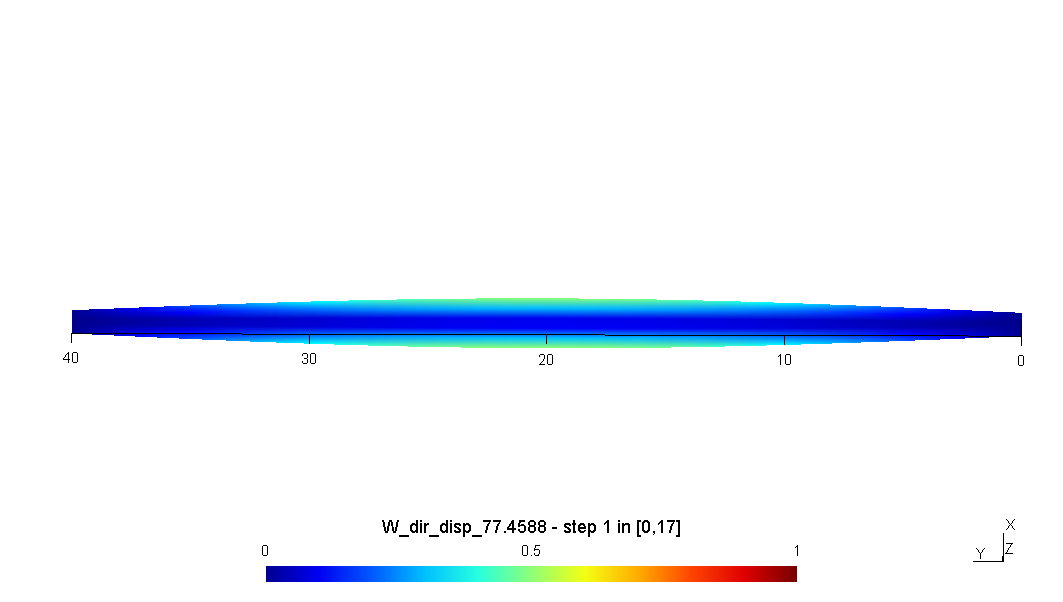
\includegraphics[width=\linewidth,trim={0 8cm 0 8cm},clip]{NAS277_pos_2.png}
%\caption{Mode Shape 2}
\end{subfigure}\vfill
\begin{subfigure}{1\textwidth}
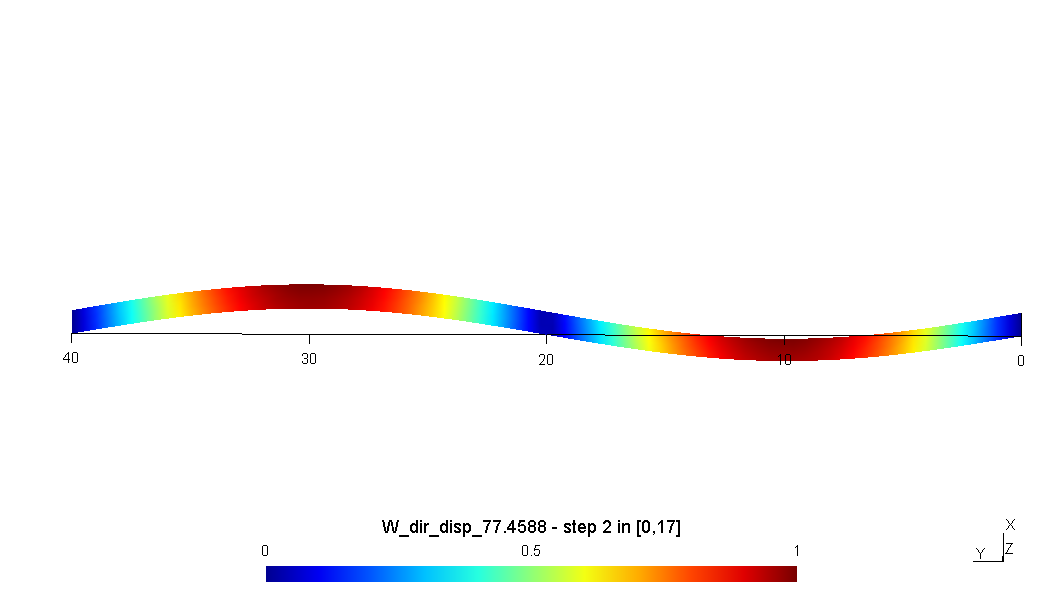
\includegraphics[width=\linewidth,trim={0 8cm 0 8cm},clip]{NAS277_pos_3.png}
%\caption{Mode Shape 3}
\end{subfigure}

%\caption{Natural Modes of a rectangular strip}
\end{figure}

Analytical Solution = 77.47 \\
Numerical Solution =  77.45\\
Error $\%$ = 0.01 $\%$.


\begin{equation*}
\begin{split}
\rho^2 \omega_{mn}^2=   D  \left[ \left( \frac{m\pi}{a} \right)^2 + \left( \frac{n\pi}{b} \right)^2 \right]\\ + N_1 \left( \frac{m\pi}{a} \right)^2 +N_2 \left( \frac{n\pi}{b} \right)^2 
\end{split}
\end{equation*}



\column{0.5\textwidth}


\begin{table}[ht]
\renewcommand{\arraystretch}{1.5}
\centering
\begin{tabular}{ll}
\hline
\multicolumn{2}{l}{Material Property} \\ \hline  \hline
Young's Modulus ($E$)          &1E11 $Pa$        \\
Poission's Ratio ($\nu$)       & 0.3            \\ 
Density($\rho$)       &     7810         \\ 
    \hline
    \multicolumn{2}{l}{Geometric Data} \\ \hline  \hline
            length ($l$)        & 1 $m$   \\
            breath ($b$)        & 40 $m$   \\
            Thickness($t$)     &         0.5 $mm$  \\
             \hline
                \multicolumn{2}{l}{Loading Data} \\ \hline  \hline
            Axial load ($N_x$)        & 6E7 $N/m^2$   \\
             \hline
\end{tabular}
\end{table}






\end{columns}
\begin{block}{Reference}
Arthur W.Leissa ,Vibration of Plates,NASA SP-160, pg:277, Ch:10.2. \\
\end{block}
\end{frame}



\begin{frame}
\frametitle{Wave Speed in the moving metal strip}
The same model used in the previous problem is also used here with additional line speed to simulate moving material.

\begin{figure}[h!]
\centering
\begin{subfigure}{1\textwidth}
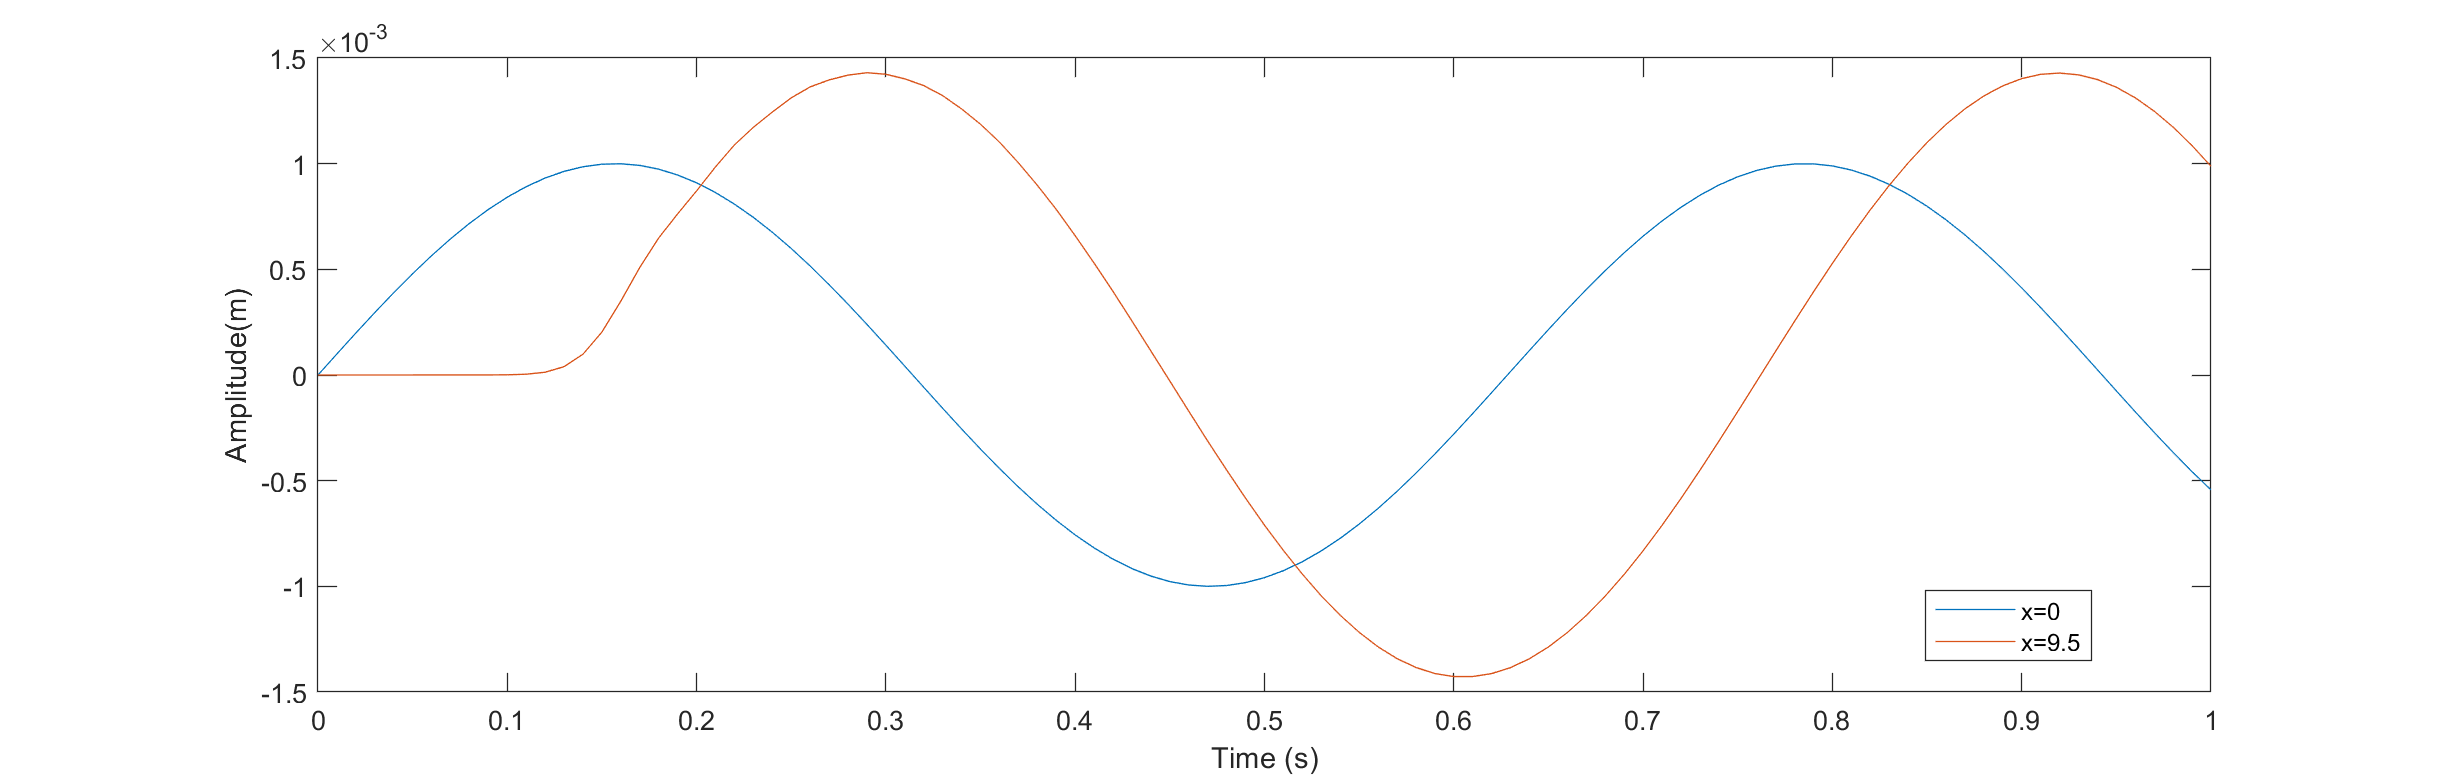
\includegraphics[width=\linewidth,trim={0 0 0 0},clip]{wavespeed.png}
%\caption{Mode Shape 1}
\end{subfigure} 

%\caption{Natural Modes of a rectangular strip}
\end{figure}
\begin{columns}

\column{0.5\textwidth}
\begin{equation*}
c=v+\sqrt{\frac{T}{m}}
\end{equation*}
 
 $T$ = Tension , $m$ = Mass per unit length, $v$ = line speed and $c$ = wave speed. 



\column{0.5\textwidth}

\begin{table}[ht]
\renewcommand{\arraystretch}{1.5}
\centering
\begin{tabular}{ll}
\hline
                \multicolumn{2}{l}{Loading Data} \\ \hline  \hline
            Line Speed ($V_1$)        &10 $m/s$   \\
             \hline
\end{tabular}
\end{table}
\end{columns}
Analytically Solution = 71.977 $ms^{-1}$, Numerical solution = 71.42 $ms^{-1}$ and The 
Error $\%$ = 0.89 $\%$.
\end{frame}

\begin{frame}
\frametitle{comparison with 1D FD model}
The same model is again employed to compare it with the existing one dimensional finite difference model.
\begin{figure}[h!]
\centering
\minipage{1\textwidth}%
  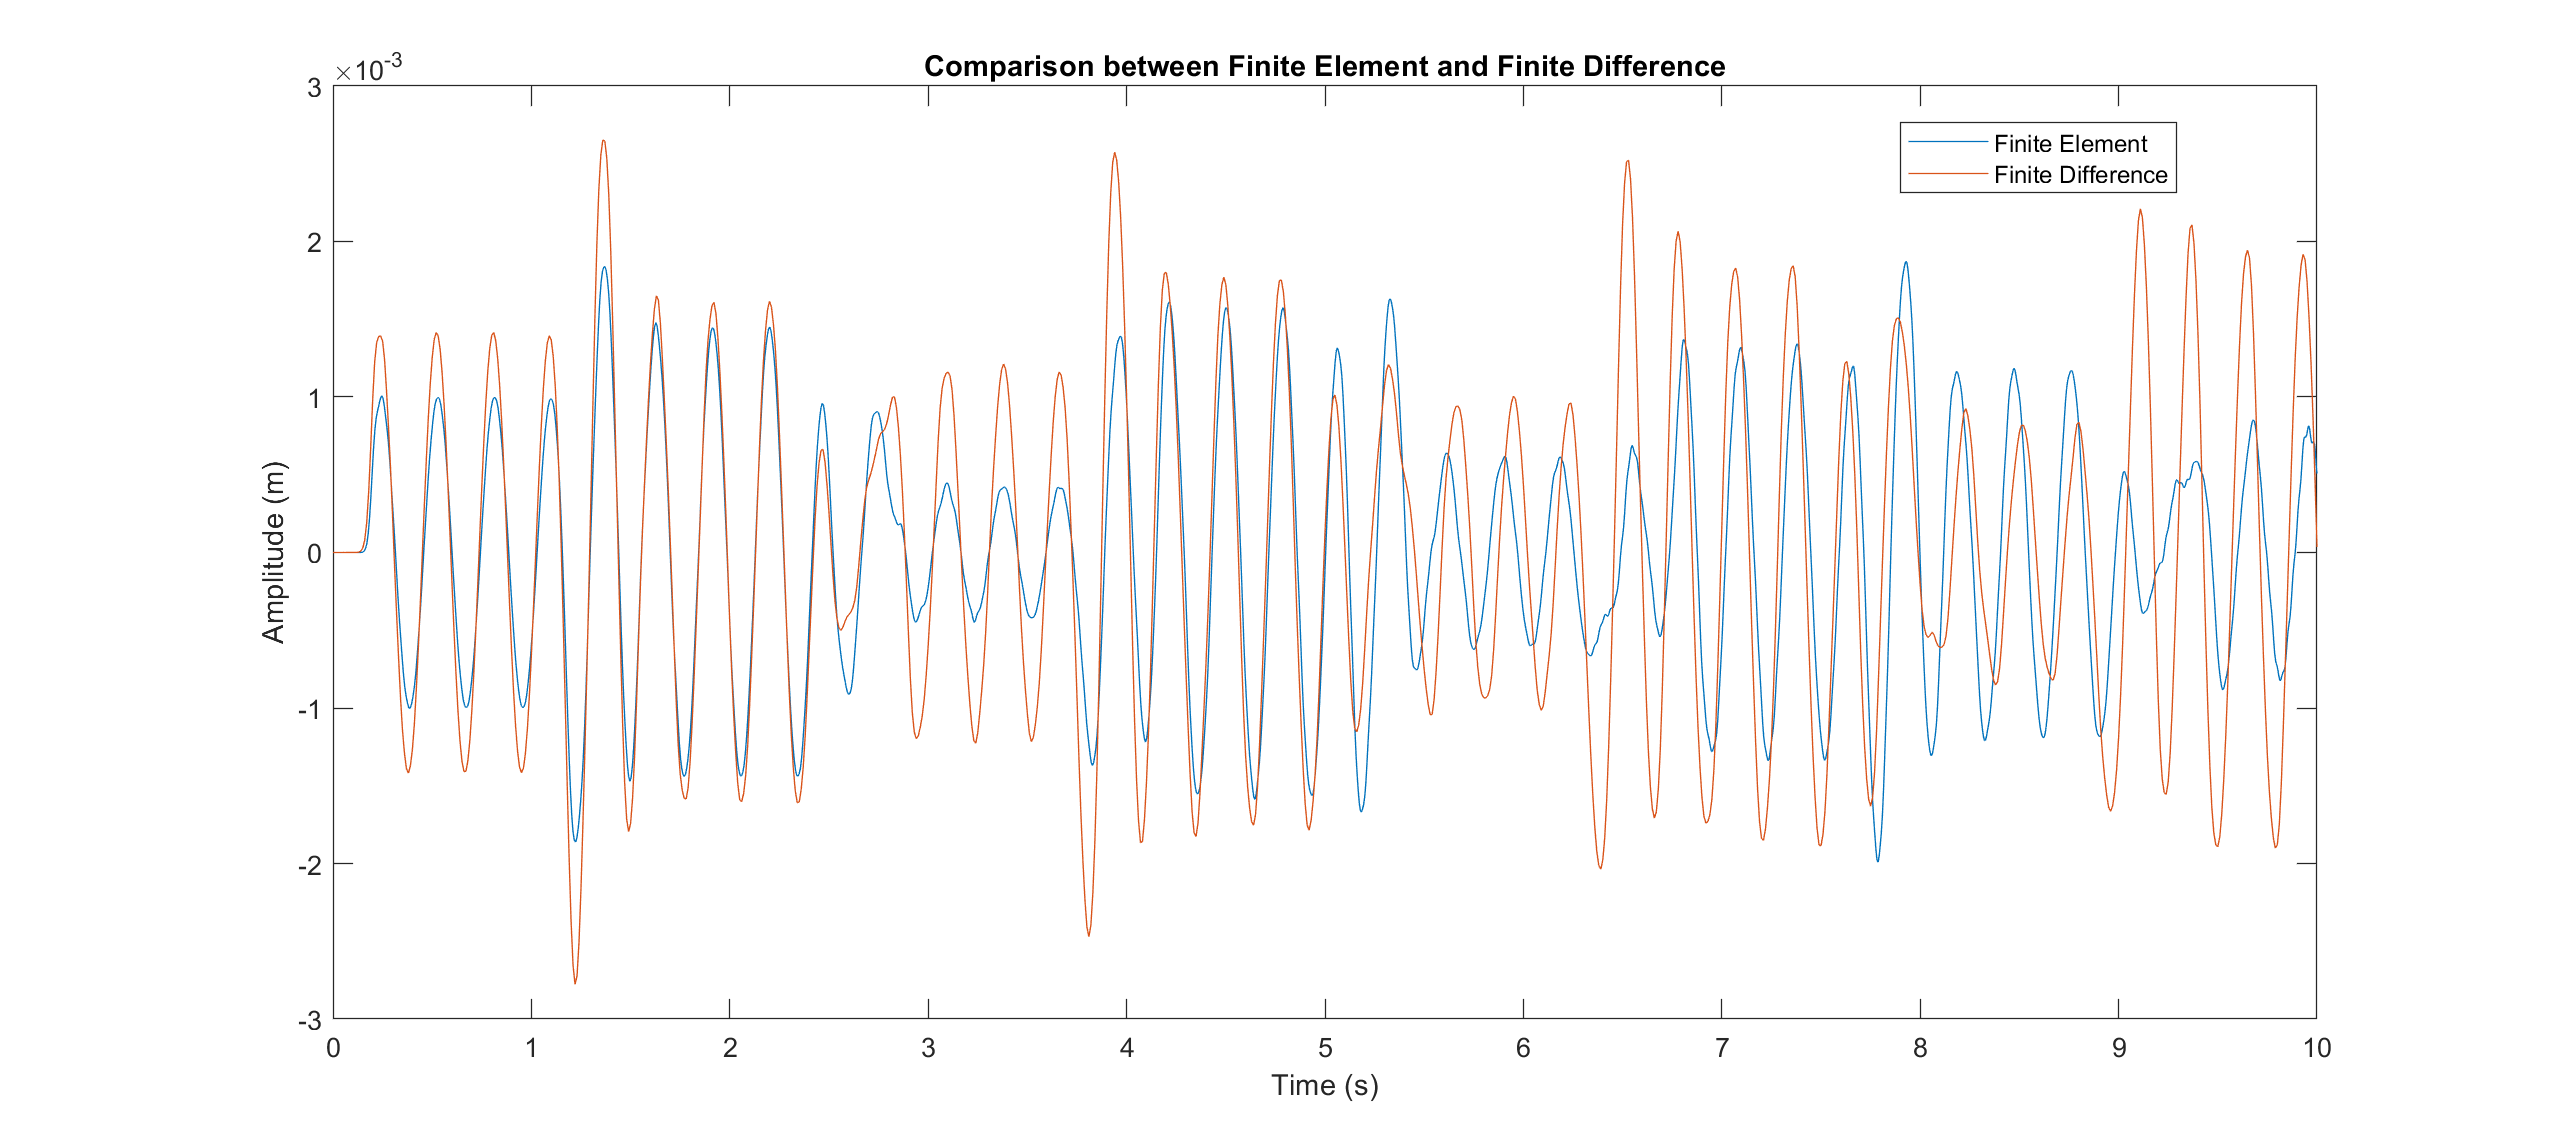
\includegraphics[width=\linewidth,trim={2cm 0 2cm 0},clip]{FdvsFe1.png}
  %\caption{FEM solution plot}\label{fig:awesome_image3}
\endminipage
\end{figure}
The displacement of the plate at the distance of 10 m from origin is plotted against time.
\end{frame}


\begin{frame}
\frametitle{Solution plot of the Dynamic Analysis}
%\movie[width=0.7\textwidth]{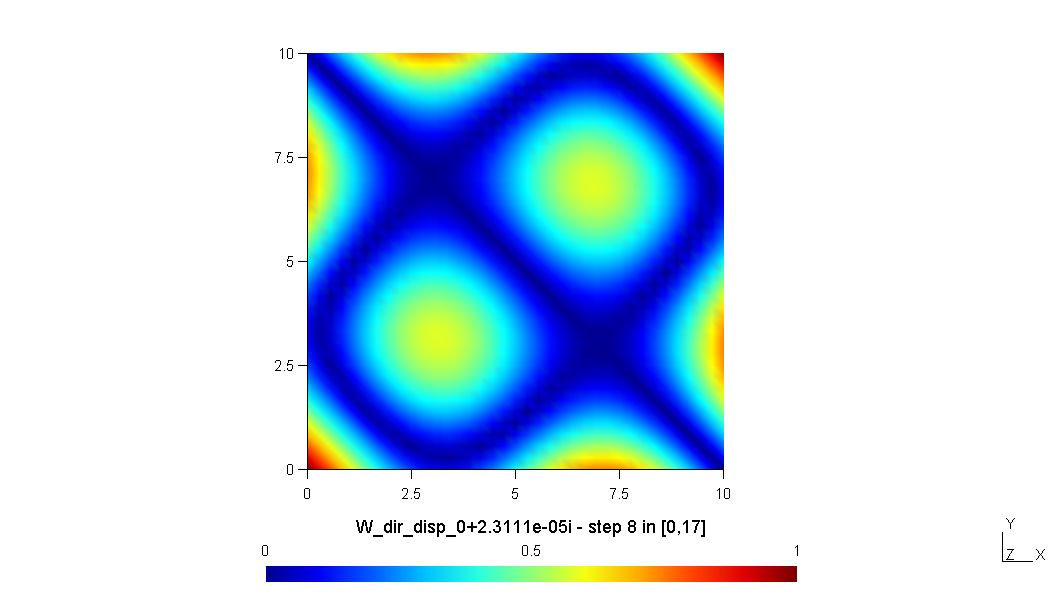
\includegraphics[width=0.7\textwidth]{VMP09_T12_pos_F9.png}}{movie1.mpg}
The solution post processing of the previous problem is provided.
\href{run:movie1.mpg}{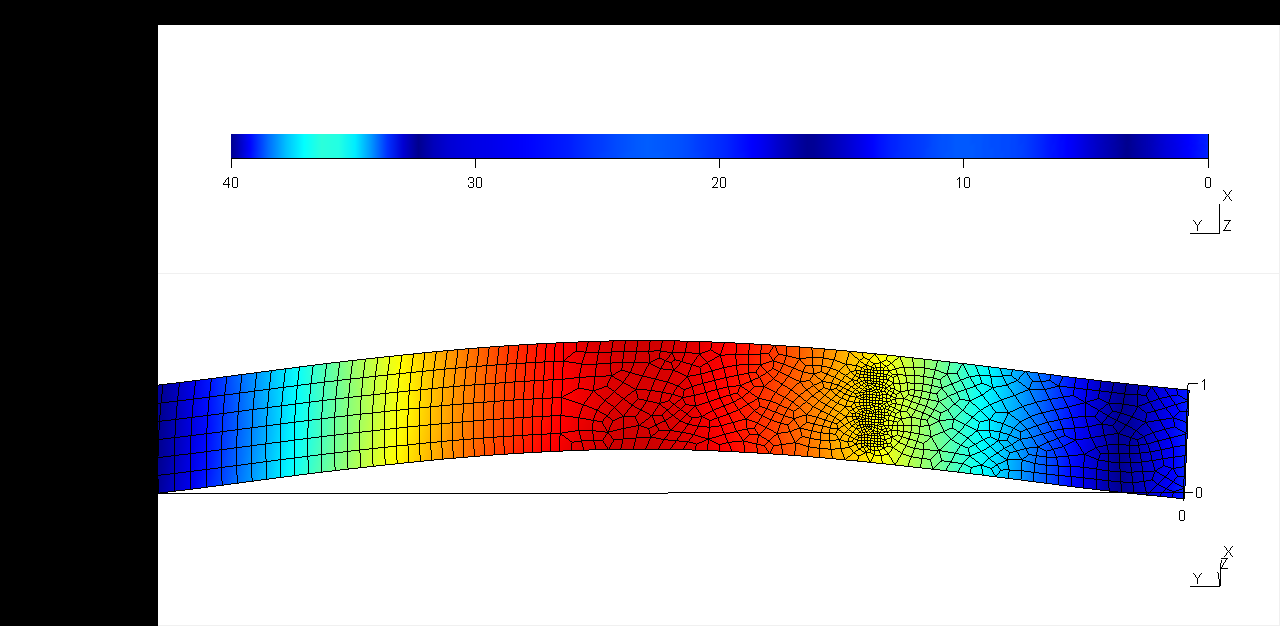
\includegraphics[width=0.4\textwidth]{movie1.png}} \\
The solution post processing of the same problem with additional time varying body forces is provided.\\
\href{run:movie2.mpg}{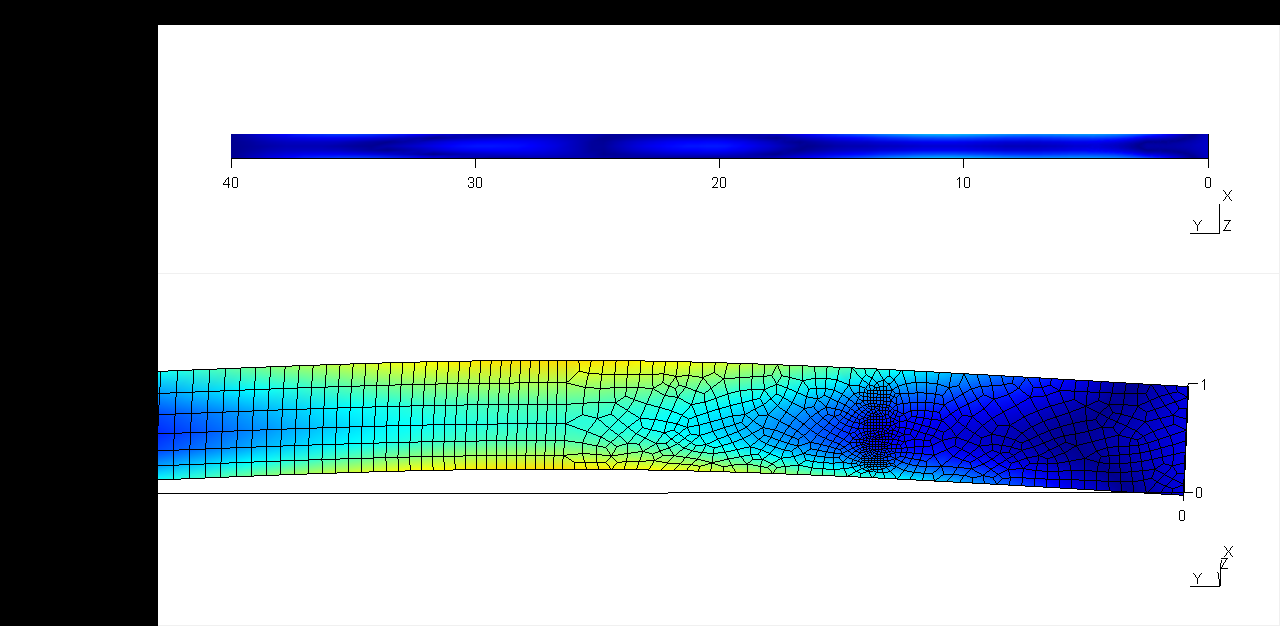
\includegraphics[width=0.4\textwidth]{movie2.png}}
\begin{block}{analysis Statistics}
nt=250 , nN = 1886 , nE = 1836, ndof = 5640 \\
Solution Time = s

\end{block}

\end{frame}

\section{Conclusion}
\begin{frame}
\frametitle{Conclusion}
\begin{block}{Advantages of FEM}
\begin{itemize}
\item Better control over accuracy.
\item Once coded successfully, It is very easy to implement even for complex geometry and mesh.
\item Higher dimensions can be easily modeled.
\end{itemize}

\end{block}

\begin{block}{Disadvantages of FEM}
\begin{itemize}
\item Computationally expensive.
\item Complexity in coding may be overwhelming .
\item Suffers from "The curse of dimensionality!".

\end{itemize}

\end{block}
\end{frame}

\begin{frame}
Thank you for your attention!!!
\end{frame}

\end{document}
